%!TEX TS-program = xelatex 
%!TEX encoding = UTF-8 Unicode
%
%  my_title
%
%  Created by David Perez on march 2010.
%  Copyright (c) David Perez 2010. All rights reserved.
%

% -*- Mode:TeX -*-



%% The documentclass options along with the pagestyle can be used to generate
%% a technical report, a draft copy, or a regular thesis.  You may need to
%% re-specify the pagestyle after you \include  cover.tex.  For more 
%% information, see the first few lines of mitthesis.cls. 

%\documentclass[12pt,vi,twoside]{mitthesis}
%%
%%  If you want your thesis copyright to you instead of MIT, use the
%%  ``vi'' option, as above.
%%
%\documentclass[12pt,twoside,leftblank]{mitthesis}
%%
%% If you want blank pages before new chapters to be labelled ``This
%% Page Intentionally Left Blank'', use the ``leftblank'' option, as
%% above. 

%For the final thesis
\documentclass[12pt,vi]{mitthesis}
\pagestyle{plain}

%for technical report
%\documentclass[12pt,vi,twoside]{mitthesis}
%\pagestyle{plain}

%for draft
%\documentclass[11pt,singlespace,draft]{mitthesis}
%\pagestyle{drafthead}


%%package for TODO lists, comments, annotations on pdf, with colors
%\usepackage[enable, spanish, colorinlistoftodos]{todonotes}
%%el comando de abajo hace el trabajo automaticamente identificando si es un
%%draft
%\usepackage[obeyDraft]{todonotes}
%%los posibles COLORES usados para \todo[color=green!40]{test12} son:
%%green, red, blue!20!white (para mezclar dos colores)
%%la UBICACION del comentario, en el borde o entre parrafos:
%%\todo[noline]{A note with no line ...} noline o line o inline
%%\missingfigure[figwidth=6cm]{Testing a long text string}

%\usepackage[pdfborder={0 0 0}]{hyperref}
\usepackage[colorinlistoftodos, textwidth=2.8cm, shadow]{todonotes}
\usepackage{amsmath}
\usepackage[displaymath, tightpage]{preview}




\usepackage{lgrind}

%% in case I include .eps versions of all figures for those w/o pdftex
%\usepackage{ifpdf}
%\ifpdf
%\usepackage[pdftex]{graphicx}
%\else
\usepackage{graphicx} 
%\fi

\usepackage{amsmath,amssymb,amsfonts} % easily align arrays of equations
\usepackage{hyperref} % hyperlinks
\usepackage{subfig} % multi-part figures
\usepackage{pdfpages} % makes it easy to insert all those nsigmapi fits


%%%%%%%%%%%%%%%%%%%%%%%%%%%%%%%%%%%%%%%%%%%%%%%%%%%%%%%%%%%%%%%%%%%%%%%%%%
%%%%Paquete usado para rotar la pagina,
%%%%encontrado en http://texblog.wordpress.com/2007/11/10/landscape-in-latex/
\usepackage{pdflscape}


%%%%%%%%%%%%%%%%%%%%%%%%%%%%%%%%%%%%%%%%%%%%%%%%%%%%%%%%%%%%%%%%%%%%%%%%%%
%%%%Paquete usado para el glosario y los acronimos,
%%%%encontrado en http://www.ctan.org/tex-archive/macros/latex/contrib/glossaries/
%\usepackage[nonumberlist]{glossaries}
%\usepackage[style=long,toc]{glossaries}
\usepackage[style=altlist, % use altlist style
            %toc, % add the glossary to the table of contents
            sanitize={description=false},% want to use description in main
            document description% acronyms have a user-supplied description
           ]{glossaries}

%\makeglossaries
%\loadglsentries{glossaries/database1}
\makeglossaries
\loadglsentries{glossaries/acronyms}
%\printglossaries





%%%%%%%%%%%%%%%%%%%%%%%%%%%%%%%%%%%%%%%%%%%%%%%%%%%%%%%%%%%%%%%%%%%%%%%%%%
%%%%%%%%%%%%%%%%%%%%begin code formatting%%%%%%%%%%%%%%%%%%%%%%%%%%%%%%%%%
%paquete para agregar codigo fuente
%\usepackage{listings}
\usepackage{listings}
\usepackage{courier}
\lstset{
         basicstyle=\footnotesize\ttfamily, % Standardschrift
         %numbers=left,               % Ort der Zeilennummern
         numberstyle=\tiny,          % Stil der Zeilennummern
         %stepnumber=2,               % Abstand zwischen den Zeilennummern
         numbersep=5pt,              % Abstand der Nummern zum Text
         tabsize=2,                  % Groesse von Tabs
         extendedchars=true,         %
         breaklines=true,            % Zeilen werden Umgebrochen
         keywordstyle=\color{red},
                frame=b,         
 %        keywordstyle=[1]\textbf,    % Stil der Keywords
 %        keywordstyle=[2]\textbf,    %
 %        keywordstyle=[3]\textbf,    %
 %        keywordstyle=[4]\textbf,   \sqrt{\sqrt{}} %
         stringstyle=\color{white}\ttfamily, % Farbe der String
         showspaces=false,           % Leerzeichen anzeigen ?
         showtabs=false,             % Tabs anzeigen ?
         xleftmargin=17pt,
         framexleftmargin=17pt,
         framexrightmargin=5pt,
         framexbottommargin=4pt,
         %backgroundcolor=\color{lightgray},
         showstringspaces=false      % Leerzeichen in Strings anzeigen ?        
 }
 \lstloadlanguages{% Check Dokumentation for further languages ...
         %[Visual]Basic
         %Pascal
         %C
         %C++
         XML
         %HTML
         Java
}
    %\DeclareCaptionFont{blue}{\color{blue}} 

  %\captionsetup[lstlisting]{singlelinecheck=false, labelfont={blue}, textfont={blue}}
\usepackage{caption}
\DeclareCaptionFont{white}{\color{white}}
\DeclareCaptionFormat{listing}{\colorbox[cmyk]{0.43, 0.35, 0.35,0.01}{\parbox{\textwidth}{\hspace{15pt}#1#2#3}}}
\captionsetup[lstlisting]{format=listing,labelfont=white,textfont=white, singlelinecheck=false, margin=0pt, font={bf,footnotesize}}

%%%%%%%%%%%%%%%%%%%%end code formatting%%%%%%%%%%%%%%%%%%%%%%%%%%%%%%%%%%%%%%%%
%%%%%%%%%%%%%%%%%%%%%%%%%%%%%%%%%%%%%%%%%%%%%%%%%%%%%%%%%%%%%%%%%%%%%%%%%%%%%%%

\begin{document}

% -*-latex-*-
% $Log: cover.tex,v $
% Revision 1.8  2008/05/13 15:02:15  jdreed
% Degree month is June, not May.  Added note about prevdegrees.
% Arthur Smith's title updated
%
% Revision 1.7  2001/02/08 18:53:16  boojum
% changed some \newpages to \cleardoublepages
%
% Revision 1.6  1999/10/21 14:49:31  boojum
% changed comment referring to documentstyle
%
% Revision 1.5  1999/10/21 14:39:04  boojum
% *** empty log message ***
%
% Revision 1.4  1997/04/18  17:54:10  othomas
% added page numbers on abstract and cover, and made 1 abstract
% page the default rather than 2.  (anne hunter tells me this
% is the new institute standard.)
%
% Revision 1.4  1997/04/18  17:54:10  othomas
% added page numbers on abstract and cover, and made 1 abstract
% page the default rather than 2.  (anne hunter tells me this
% is the new institute standard.)
%
% Revision 1.3  93/05/17  17:06:29  starflt
% Added acknowledgements section (suggested by tompalka)
% 
% Revision 1.2  92/04/22  13:13:13  epeisach
% Fixes for 1991 course 6 requirements
% Phrase "and to grant others the right to do so" has been added to 
% permission clause
% Second copy of abstract is not counted as separate pages so numbering works
% out
% 
% Revision 1.1  92/04/22  13:08:20  epeisach

% NOTE:
% These templates make an effort to conform to the MIT Thesis specifications,
% however the specifications can change.  We recommend that you verify the
% layout of your title page with your thesis advisor and/or the MIT 
% Libraries before printing your final copy.
\title{An Optimizing Compiler for Low-Level Floating Point Operations}

\author{Lucien William Van Elsen}
% If you wish to list your previous degrees on the cover page, use the 
% previous degrees command:
%       \prevdegrees{A.A., Harvard University (1985)}
% You can use the \\ command to list multiple previous degrees
%       \prevdegrees{B.S., University of California (1978) \\
%                    S.M., Massachusetts Institute of Technology (1981)}
\department{Department of Electrical Engineering and Computer Science}

% If the thesis is for two degrees simultaneously, list them both
% separated by \and like this:
% \degree{Doctor of Philosophy \and Master of Science}
\degree{Bachelor of Science in Computer Science and Engineering}

% As of the 2007-08 academic year, valid degree months are September, 
% February, or June.  The default is June.
\degreemonth{June}
\degreeyear{1990}
\thesisdate{May 18, 1990}

%% By default, the thesis will be copyrighted to MIT.  If you need to copyright
%% the thesis to yourself, just specify the `vi' documentclass option.  If for
%% some reason you want to exactly specify the copyright notice text, you can
%% use the \copyrightnoticetext command.  
%\copyrightnoticetext{\copyright IBM, 1990.  Do not open till Xmas.}

% If there is more than one supervisor, use the \supervisor command
% once for each.
\supervisor{William J. Dally}{Associate Professor}

% This is the department committee chairman, not the thesis committee
% chairman.  You should replace this with your Department's Committee
% Chairman.
\chairman{Arthur C. Smith}{Chairman, Department Committee on Graduate Theses}

% Make the titlepage based on the above information.  If you need
% something special and can't use the standard form, you can specify
% the exact text of the titlepage yourself.  Put it in a titlepage
% environment and leave blank lines where you want vertical space.
% The spaces will be adjusted to fill the entire page.  The dotted
% lines for the signatures are made with the \signature command.
\maketitle

% The abstractpage environment sets up everything on the page except
% the text itself.  The title and other header material are put at the
% top of the page, and the supervisors are listed at the bottom.  A
% new page is begun both before and after.  Of course, an abstract may
% be more than one page itself.  If you need more control over the
% format of the page, you can use the abstract environment, which puts
% the word "Abstract" at the beginning and single spaces its text.

%% You can either \input (*not* \include) your abstract file, or you can put
%% the text of the abstract directly between the \begin{abstractpage} and
%% \end{abstractpage} commands.

% First copy: start a new page, and save the page number.
\cleardoublepage
% Uncomment the next line if you do NOT want a page number on your
% abstract and acknowledgments pages.
% \pagestyle{empty}
\setcounter{savepage}{\thepage}
\begin{abstractpage}
% $Log: abstract.tex,v $
% Revision 1.1  93/05/14  14:56:25  starflt
% Initial revision
% 
% Revision 1.1  90/05/04  10:41:01  lwvanels
% Initial revision
% 
%
%% The text of your abstract and nothing else (other than comments) goes here.
%% It will be single-spaced and the rest of the text that is supposed to go on
%% the abstract page will be generated by the abstractpage environment.  This
%% file should be \input (not \include 'd) from cover.tex.
In this thesis, I designed and implemented a compiler which performs
optimizations that reduce the number of low-level floating point operations
necessary for a specific task; this involves the optimization of chains of
floating point operations as well as the implementation of a ``fixed'' point
data type that allows some floating point operations to simulated with integer
arithmetic.  The source language of the compiler is a subset of C, and the
destination language is assembly language for a micro-floating point CPU.  An
instruction-level simulator of the CPU was written to allow testing of the
code.  A series of test pieces of codes was compiled, both with and without
optimization, to determine how effective these optimizations were.

\end{abstractpage}

% Additional copy: start a new page, and reset the page number.  This way,
% the second copy of the abstract is not counted as separate pages.
% Uncomment the next 6 lines if you need two copies of the abstract
% page.
% \setcounter{page}{\thesavepage}
% \begin{abstractpage}
% % $Log: abstract.tex,v $
% Revision 1.1  93/05/14  14:56:25  starflt
% Initial revision
% 
% Revision 1.1  90/05/04  10:41:01  lwvanels
% Initial revision
% 
%
%% The text of your abstract and nothing else (other than comments) goes here.
%% It will be single-spaced and the rest of the text that is supposed to go on
%% the abstract page will be generated by the abstractpage environment.  This
%% file should be \input (not \include 'd) from cover.tex.
In this thesis, I designed and implemented a compiler which performs
optimizations that reduce the number of low-level floating point operations
necessary for a specific task; this involves the optimization of chains of
floating point operations as well as the implementation of a ``fixed'' point
data type that allows some floating point operations to simulated with integer
arithmetic.  The source language of the compiler is a subset of C, and the
destination language is assembly language for a micro-floating point CPU.  An
instruction-level simulator of the CPU was written to allow testing of the
code.  A series of test pieces of codes was compiled, both with and without
optimization, to determine how effective these optimizations were.

% \end{abstractpage}

\cleardoublepage

\section*{Acknowledgments}

This is the acknowledgements section.  You should replace this with your
own acknowledgements.

%%%%%%%%%%%%%%%%%%%%%%%%%%%%%%%%%%%%%%%%%%%%%%%%%%%%%%%%%%%%%%%%%%%%%%
% -*-latex-*-


\pagestyle{plain}
  % -*- Mode:TeX -*-
%% This file simply contains the commands that actually generate the table of
%% contents and lists of figures and tables.  You can omit any or all of
%% these files by simply taking out the appropriate command.  For more
%% information on these files, see appendix C.3.3 of the LaTeX manual. 


\tableofcontents
\newpage
\printglossaries
%\printglossary[title={Acronyms}]
\newpage
\listoffigures
\newpage
\listoftables






%\\.
%\\. 
%\\.
%\\.
%\todo[inline]{Agregar la secci\'on del cover}
%	Debo agregar una hoja donde indique que estos cap\'itulos son
%	el marco teorico de la investigaci\'on, dicho comando para
%	agregar la palabra parte A por ejemplo, sin numeraci\'on de 
%	paginas en esta, voy a encontrar en el formato de tesis 
%	de la universidad de washintong basado en la del MIT, 
%	dicho template esta en mis archivos de Google Docs



\chapter*{Annotations}

Auxiliary chapter (not is part of this document content).
En esta parte explico sobre la plataforma latex que utilizo, sobre la
sistematizaci\'on que utilizo para redactar este documento, por ejemplo, que
significan los comentarios que hago con el comando TODO, etc.

\section{Convenci\'on de colores para los comentarios hechos en este documento}
	Un comentario de color 
	\emph{NARANJADO}
	\todo{Ejemplo}   
	indica las cosas que me faltan hacer.\\

	Un comentario de color 
	\emph{VERDE CLARO}
	\todo[color=green!40]{green!40}
	indica en que parte de la norma IEC 61850 se est\'a utilizando la teor\'ia
	comentada. Indica la relaci\'on del contenido bibliogr\'afico de conceptos con
	la norma. 
	Un ejemplo de uso de este tipo de comentarios en mi trabajo:
	En redes, cuando hablo de un concepto, por ejemplo, \emph{network
	reliability}, eso se habla en la norma, en la parte IEC 61850-xx, entonces yo
	indico en el comentario de que ese concepto se menciona en la tesis. 
	Esto es \'util para mi pues me sirve para justificar por que inclu\'i la 
	descripci\'on de alg\'un concepto en el trabajo, principalmente en el marco
	te\'orico, que utilizar\'e para describir todos los conocimientos necesarios
	para abordar la norma (por ejemplo: Redes, Programaci\'on orientada a
	objetos, UML).\\
	
	Los colores en \emph{LILA}
	\todo[inline, color=blue!50!red!50]{color=blue!50!red!50}
	indican peque\~nas variaciones de palabras que podr\'ia hacer pero no son de
	alta prioridad ni obligatorias de corregir (a mi punto de vista), pero
	la modificaci\'on de las partes comentadas mejorar\'ia la redacci\'on del
	texto, o bien explican por que hice esas mejoras o ubique, redacte, 
	o modifique de esa 	manera un determinado parrafo.
	

\section{Im\'agenes por agregar al trabajo}
	Por convenci\'on, utilizar\'e la siguiente imagen
	\missingfigure[color=green!40]{prueba del comando de falta de figura}
	para indicar de que est\'a faltando incluir la imagen en este lugar. Durante
	el proceso de redacci\'on se ir\'a agregando el contenido faltante




%%Agrega la lista de cosas (comentarios) que hay que hacer
\listoftodos



\chapter{Work Research Overview}

%\include{chapters/sample}
\section{Introduction}
For comming\ldots
%\section{Introduction}

Energy worldwide is at least a seven trillion dollar
a year business and expanding. Energy profoundly affects 
our economy, society, and environment \cite{Dukert:2009ab}, 
then, they are a continously researching about new technologies 
and standards in the electrical power systems, in areas such as 
information automation, related cyber security and data 
transfer performance through Smart Grids.

La energ\'ia en todo el mundo mueve por lo menos 7 billones de 
d\'olares anuales, y es un negocio en expansi\'on. Por ello, la 
energ\'ia afecta profundamente nuestra econom\'ia, sociedad y 
entorno \cite{Dukert2009}, debido a esto, existe una constante 
investigaci\'on, y han surgido nuevas tecnolog\'ias y est\'andares 
en los sistemas de potencia, en \'areas como la automatizaci\'on 
y tratamiento de la informaci\'on, por dar unos ejemplos, con el
objetivo de mejorar el performance y la seguridad en el sistema 
de potencia, a trav\'es de redes inteligentes (Smart Grids).

In the lasts years,  the power systems automation over the world
uses microprocessors embedded devices 
\cite{Santoso:2000, Schwarz:2000mc} called
Intelligent Electronic Devices (IEDs) that suport 
network communication technologies with
the aim of to send or receive information from or to many sources
to monitoring, control and supervise the generation, transmission 
and distribution of the energy. 

En los \'ultimos a\~nos, la automatizaci\'on de sistemas de potencia 
en todo el mundo utiliza ampliamente dispositivos basados en uno o 
varios microprocesadores \cite{Santoso:2000, Schwarz:2000mc} integrados 
llamados Intelligent Electronic Devices (IEDs)  que utilizan 
tecnolog\'ias de redes de comunicaci\'on con el objetivo de enviar 
o recibir informaci\'on de o para varias fuentes con el objetivo 
de monitorear, controlar, y supervisar la generaci\'on, transmisi\'on 
y distribuci\'on de la energ\'ia
   \cite{McDonald:2007, IEEE:1997dic, Schwarz:2008wi}.

The information interchagebility between IEDs from diferent
vendors was coming complex, expensive, and sometimes 
impossible, then the industry 

\ldots\ldots\ldots

to adopt the IEC 61850 standard to achieve the interoperability, 
realiability and more quality for the information interchange 
of the Energy Management System (EMS).

\ldots\ldots\ldots aca debo colocar las siglas de EMS, ver como
arreglar este tema para que quede todo bien el tema de las siglas
  

El intercambio de informaci\'on entre IEDs de diferentes fabricantes 
se ha vuelto muy complejo, costoso, y a veces imposible, es por ello 
que la industria se ha puesto de acuerdo para adoptar el est\'andar 
IEC 61850 y as\'i conseguir interoperabilidad, confiabilidad y mayor 
calidad en el intercambio de informaci\'on dentro del Sistema de 
Gerenciamiento de Energ\'ia (EMS-Energy Management System). 

The IEC 61850 standard ``Comunication Networks and Systems in Substations" 
provide a support for sustainable interoperability between IEDs: 
information model, information interchange methods, communications 
protocols mappings and a Substation Configuration Language (SCL) 
for electrical energy systems (Generation, Transmission and Distribution) 
for hight, might and low voltage \cite{Schwarz2008}. 

La norma IEC 61850 ``Comunication Networks and Systems in Substations" 
provee un perfecto soporte para una interoperabilidad sustentable entre 
IEDs: modelado de la informaci\'on, m\'etodos para intercambio de la 
informaci\'on, mapeo a protocolos de comunicaci\'on, y un lenguaje de 
configuraci\'on de subestaciones (SCL) para sistemas el\'ectricos de 
energ\'ia (Generaci\'on, Transmisi\'on y Distribuci\'on para alta, 
media y baja tensi\'on) \cite{Schwarz2008}. 

Initially, the standard IEC 61850 focuses on substations, 
and now it are extended to 

\ldots\ldots\ldots satisfacer no se decir..

the totality of the 

La norma IEC 61850, en la actualidad, no se enfoca \'unicamente a 
subestaciones, tambi\'en es aplicable y extensible para satisfacer 
las necesidades de casi la totalidad de la cadena de suministro de 
energ\'ia, entre los cuales destacamos la protecci\'on de l\'ineas de 
transmisi\'on, plantas de energ\'ia e\'olica, distribuci\'on de 
energ\'ia y centrales hidroel\'ectricas, sistemas fotovoltaicos y 
coches el\'ectricos \cite{Schwarz2005, DER2009, German2009}. 

El modelado jer\'arquico de la informaci\'on a trav\'es de nodos 
l\'ogicos es una cuesti\'on clave. La agrupaci\'on correcta de los 
nodos l\'ogicos representan funciones o equipos utilizados en los 
sistemas de potencia. Cada nodo l\'ogico provee una lista de informaci\'on 
bien designada y organizada. Los objetos y servicios definidos en la parte 
IEC 61850-7-2 de la norma permiten el intercambio de esta 
informaci\'on \cite{TC572004}.

En julio del 2007 las extensiones de los nodos l\'ogicos a centrales 
hidroel\'ectricas han sido aprobadas, publicadas y est\'an listas 
para su uso, en el apartado IEC 61850-7-4-10: 
\emph{Hydroelectric Power Plants - Communication for monitoring and control}; 
agregando 60 nodos l\'ogicos y 350 \emph{Data Objects} a la serie 
IEC 61850 \cite{IEC61850TC57, Schwarz2008b}.

Este trabajo consiste en la aplicaci\'on de la norma IEC 61850, 
en especial del modelado de nodos l\'ogicos definidos en la parte 
7-4-10 Hydro Power Plants y de los objetos y servicios de comunicaci\'on 
para la automatizaci\'on de una unidad generadora t\'ipica de Itaipu, 
y proponer al TC57 (International Electrotechnical Commission, Technical 
Committee 57) la complementaci\'on o extensi\'on de nodos l\'ogicos de 
la norma que actualmente son insuficientes para las unidades generadoras 
de Itaipu. Como estudio de caso, se modelar\'an los nodos l\'ogicos y 
servicios de comunicaci\'on necesarios para el regulador de velocidad de 
la unidad generadora. Este trabajo de investigaci\'on se basa en el \'item 
del documento ``Proposta de Temas para Monografias de 
Especializa\c c\~ao - Automa\c c\~ao, Controle e Supervis\~ao do 
Processo el\'etrico Baseado na Norma  IEC 61850 -  A-4 - Automa\c c\~ao 
de Unidades Geradoras - Modelagem Completa da Unidade Geradora" de la 
Itaipu Binacional, redactado por Marcos Fonseca Mendes, Antonio Sertich 
Koehler, Ladislao Aranda Arriola, funcionarios de la Itaipu Binacional. 

\section{Aim of this Research}
Blah blah blah

\section{Research Methodologies and Techniques}
	\todo[inline]{
		Falta traducir al ingl\'es toda esta secci\'on.
		Esta secci\'on la extraje de mi anteproyecto, que originalmente fue escrita
		en espa\~nol.
		}
	\subsection{Investigaci\'on bibliogr\'afica} 
		Incluye la investigaci\'on y estudio de la norma IEC 61850, en especial las
		definiciones de modelos de informaci\'on definidos en la parte IEC
		61850-7-4-10 \emph{Basic communication structure for substation and feeder
		equipment – Compatible logical node classes and data classes - Hydro Power
		Plants}, los servicios de intercambio de informaci\'on para diferentes
		funciones (por ejemplo, control, reporte, \emph{getters} y \emph{setters})
		definidos en el apartado IEC 61850-7-2 \emph{Basic communication structure
		for substation and feeder equipment – Abstract communication service
		interface (ACSI)}, la implementaci\'on de dichos servicios de comunicaci\'on
		a trav\'es de protocolos especificados en la parte IEC 61850-8-1
		\emph{Specific Communication Service Mapping (SCSM) – Mappings to MMS (ISO
		9506-1 and ISO 9506-2) and to ISO/IEC 8802-3} para las necesidades de la
		unidad generadora, y otros documentos, normas, y tecnolog\'ias relacionadas.
	\subsection{Investigaci\'on de campo}
		Incluye el levantamiento de informaciones del generador de Itaip\'u, la
		identificaci\'on de las funciones de automatizaci\'on inherentes regulador de
		velocidad de la unidad generadora y otras documentaciones y estad\'isticas
		relacionadas al caso en estudio. Tambi\'en incluye la simulaci\'on en una
		red IEC 61850 utilizando las herramientas de ingenier\'ia disponibles en el
		mercado para tal efecto.
	\subsection{Creaci\'on de los objetos}
		Dise\~no de los nodos l\'ogicos normalizados en la parte IEC 61850-7-4, e
		IEC 61850-7-4-10 mediante UML, implementaciones en XML, Java, C++, o
		mediante las herramientas de ingenier\'ia especializadas en la norma IEC
		61850 disponibles en el mercado.
	\subsection{Identificaci\'on de servicios de informaci\'on}
		Modelado completo de los servicios de comunicaci\'on necesarios para el
		regulador de velocidad de una unidad generadora t\'ipica de Itaipu
		utilizando la parte IEC 61850-7-2.
	\subsection{Propuesta de extensi\'on/complementaci\'on de los nodos l\'ogicos
		e ICDs} Por ejemplo, ZAXN, insuficiente para la alimentaci\'on AC y DC de los
		servicios auxiliares de Itaipu.
	\subsection{Estructuraci\'on de una metodolog\'ia de aplicaci\'on de la norma
		IEC 61850 en la automatizaci\'on de hidroel\'ectricas} Elecci\'on de las
		herramientas de ingenier\'ia disponibles en el mercado y que mejor se adapten
		a la automatizaci\'on de unidades generadoras aplicando la norma IEC 61850 y
		la creaci\'on de procedimientos padronizados utilizando dichas herramientas,
		para satisfacer los requerimientos de ingenier\'ia definidos en el apartado
		IEC 61850-4 subsecci\'on 3, y para identificar las funciones de
		automatizaci\'on que son necesarias para el modelado de los nodos l\'ogicos,
		pero no est\'an contempladas en la norma IEC 61850.

\section{Originality of this Research}
For comming\ldots
\section{Organization of this Research Document}
Blah blah blah 

\chapter{Introduction to the IEC 61850 series}
For comming\ldots  

List of the IEC 61850 parts considered 
in this work: \todo{o por considerar} \\
IEC61850-1:2003 	\cite{IEC61850-1:2003} \\
IEC61850-2:2003		\cite{IEC61850-2:2003} \\
IEC61850-3:2002		\cite{IEC61850-3:2002} \\
IEC61850-4:2002		\cite{IEC61850-4:2002} \\
IEC61850-5:2003		\cite{IEC61850-5:2003} \\
IEC61850-6:2004		\cite{IEC61850-6:2004}  \\
IEC61850-7-1:2003	\cite{IEC61850-7-1:2003} \\
IEC61850-7-2:2003	\cite{IEC61850-7-2:2003} \\
IEC61850-7-3:2003	\cite{IEC61850-7-3:2003} \\
IEC61850-7-4:2003	\cite{IEC61850-7-4:2003} \\
IEC61850-7-410:2007	\cite{IEC61850-7-410:2007} \\
IEC61850-7-420:2009	\cite{IEC61850-7-420:2009} \\
IEC61850-7-430:200-X\cite{IEC61850-7-430:200-X} \\
IEC61850-7-5:2010	\cite{IEC61850-7-5:2010} \\
IEC61850-7-500:2010	\cite{IEC61850-7-500:2010} \\
IEC61850-7-510:2009	\cite{IEC61850-7-510:2009} \\
IEC61850-7-520:2010	\cite{IEC61850-7-520:2010} \\
IEC61850-7-10:2009	\cite{IEC61850-7-10:2009} \\
IEC61850-8-1:2004	\cite{IEC61850-8-1:2004} \\
IEC61850-9-1:2003	\cite{IEC61850-9-1:2003} \\
IEC61850-9-2:2004	\cite{IEC61850-9-2:2004} \\ 

\todo{debo arreglar las bibliografias del bibtex, 
no se estan viendo como se debe}

%%hello world!  first commit from linux! - this is a test

%%Este capítulo debe ser el primer tema técnico a tratar,
%%debido a que mi tema se trata al modelado de objetos 
%%y de servicios de comunicación (al final los servicios
%%de comunicación se modelan como objetos via xml)
%%y también la utilización de interfaces da una buena base
%%para entender las capas del modelo OSI: las interfaces
%%que posee cada capa para comunicarse con las otras
%%(servicios) son muy bien compreendidas una vez
%%tratada el tema de interfaces de OOP. Al final, 
%%este tema de interfaces es 
%%abstracción, tratada en ingeniería de software. Por 
%%ello, es un buen punto empezar desde aquí.

\chapter{Object-oriented programming}

\section{Introduction}

The IEC 61850 information model 
is classified as a  
\glsentrytext{O-O} system. Is necessary 
to have a clear understanding of \gls{O-O} technology
to dive into IEC 61850 object modelling. 
For this reason this chapter describes 
the \gls{O-O} technology
on which the IEC 61850 information model 
has been standarized\todo[inline]{No se si esta 
bien escrita la palabra standarized}. 

The chapter does not describe all the \gls{O-O} principles, 
just \todo{�trans:just focuses or focuses just?} focuses 
on the neccesary
background to understand the IEC 61850 
information model. 
The sections which follow will define the 
background which the IEC 61850 
object oriented information system 
was constructed, both formally 
and through examples.
\todo[inline]{debo agregar las abreviaciones de O-O
a mi glossaries package}
A detailed description of the \gls{O-O} fundamentals  
and reference materials are provided. To achieve a 
robust concepts comprehension a practical 
implementation with the%the Unified Modeling Language 
\gls{UML} 
\todo{agregar al glossaries} 
\cite{UML2:2009} 
and Java \cite{Java:specification} are provided. 
This chapter is very
practical in the sense that uses language programmings to model 
very carefully selected models  
used by the IEC 61850 standard, 
(but not explaining explicitly nothing 
about the standard yet!).
This chapter is destined 
for electrical engineers and professionals of 
related areas readers which the \gls{O-O} software construction 
is not part of the curriculum. For this reason, 
the practical examples uses electricity area 
elements. The readers with a strong knowledge 
of programming could skip this
chapter \todo[inline, color=blue!50!red!50]{
	deber\'ia agregar esta ultima frase?:
	\emph{The readers with a strong knowledge 
	of programming could skip this
	chapter}
}




\todo[inline]{En este cap�tulo voy a agregar 
los graficos a continuacion:

(los ejemplos que voy usando son con estas clases)}


\begin{figure}
  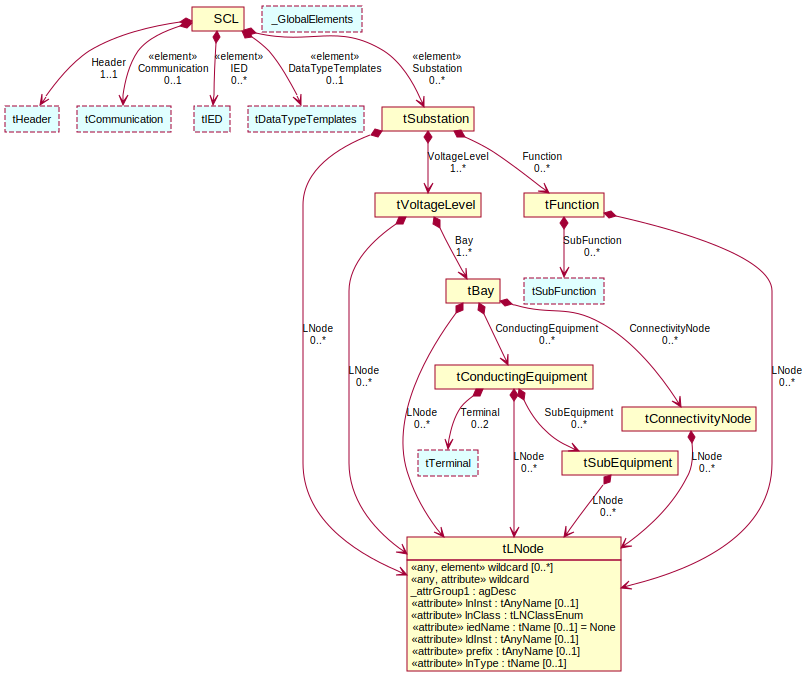
\includegraphics[width=1.0\textwidth]{chapters/ch-oop/figures/LogicalNodeAllocationStructure}
  \caption{Logical Node and their role at the substation level}
  \label{fig:LogicalNodeAllocationStructure}
\end{figure}

\begin{landscape}
	\begin{figure}	
	  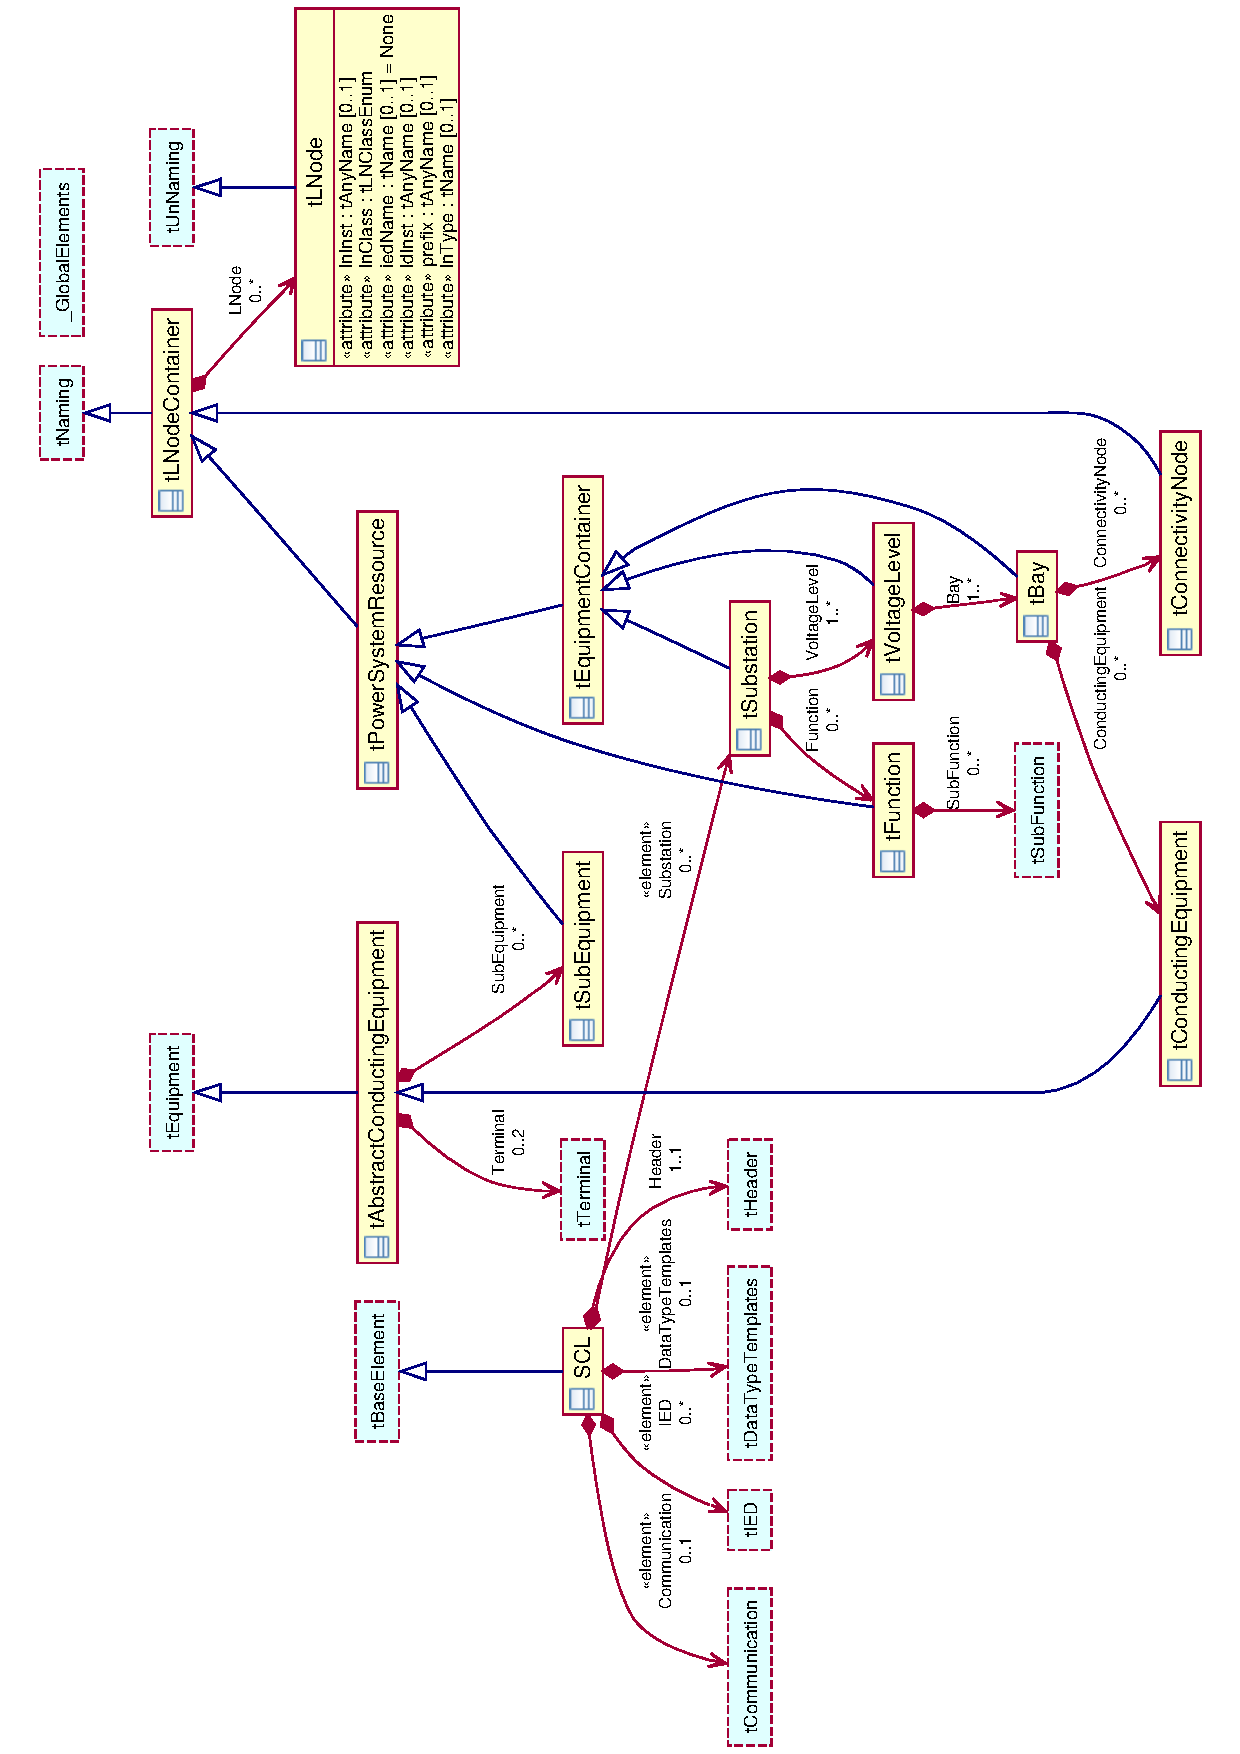
\includegraphics[angle=-90, width=1.0\linewidth]{chapters/ch-oop/figures/LogicalNodeAllocationStructure_with_heritance}
	  \caption{Logical Node and their role at the substation level, depicted with
	  the heritance details}
	  \label{fig:LogicalNodeAllocationStructure_with_heritance}
	\end{figure}
\end{landscape}
	
\section{Basics of object-oriented programming}

\subsection{Introduction to object-oriented programming}

%TODO: citar
%esta parte fue obtenida del libro de adobe, del cap 5. 
Object-oriented programming (OOP) is a way of organizing the code 
in a program by grouping it into objects-individual elements that include 
information (data values) and functionality. Using an 
object-oriented approach to organizing a program allows 
you to group particular pieces of information (for 
example, a automation function or a current value) together with 
common functionality or actions associated with that 
information (such as ``switchgear actuation'' or 
``voltage measurement''). These items are combined into a single 
item, an object (for example, an 
\todo[size=\tiny]{cambiar por un ejemplo el\'ectrico}
``Album'' or ``MusicTrack''). Being 
able to bundle these values and functions together provides several 
benefits, including only needing to keep track of a single 
variable rather than multiple ones, organizing related 
functionality together, and being able to structure 
programs in ways that more closely match the real world.  


\subsection{Common object-oriented programming tasks}

%Aca va la pagina 99 de actionscript programming.
In practice, 
%citar las prácticas comunes
\begin{itemize}
	\item Defining classes
	\item Creating properties, methods, and get and set accessors (accessor
	methods) 
	\item Controlling access to classes, properties, methods, and accessors
	\item Creating static properties and methods
	\item Creating enumeration-like structures
	\item Defining and using interfaces
	\item Working with inheritance, including overriding class elements 
\end{itemize}



\section{Classes}

A class is a static 
%off-line \todo{es realmente off-line?}
template from which objects are 
created. Classes are used 
to classify objects thanks 
that its defines 
common operations 
and a data structure, 
and the types of 
datas that the object can 
store.\\


%Codigo fuente
%C:\Documents and Settings\DELL\Mis
%documentos\tesismayo\tesismayo\thesis\chapters\ch-oop\source\java\src\HelloWorld.java
%\lstinputlisting[label=samplecode,caption=A sample]{sourceCode/HelloWorld.java}
%chapters\ch-oop\source\java\src\HelloWorld.java
\lstinputlisting[label=codeClass,
caption=Class in Java]{chapters/ch-oop/source/java/src/SERVER_v1.java}

%%TODO: cite adobe book

\subsection{Attributes}
\todo[inline]{completar esta parte}
	\lstinputlisting[label=codeAttributes,
	caption=Class with attributes in Java]
	{chapters/ch-oop/source/java/src/SERVER_v2.java}



\subsection{Methods}
Methods are functions that are part of a class 
definition. Once an instance of the class is created, 
a method is bound to that instance.\\
	\lstinputlisting[label=codeMethod,
	caption=Class with attributes and methods in Java]
	{chapters/ch-oop/source/java/src/SERVER_v3.java}



	\subsubsection{Get and set accessor methods}
	Get and set accessor functions, also called getters 
	and setters, allow you to adhere to the programming principles of 
	information hiding and encapsulation while providing an 
	easy-to-use programming interface for the classes that you 
	create. Get and set functions allow you to keep your class 
	properties private to the class, but allow users of your class 
	to access those properties as if they were accessing a 
	class variable instead of calling a class method. 
	The advantage of this approach is that you can avoid 
	having two public-facing functions for each property 
	that allows both read and write access. \\

		\lstinputlisting[label=codeMethod,
		caption=Class with attributes, methods, getters and setters in Java]
		{chapters/ch-oop/source/java/src/SERVER_v4.java}
	
	
	\subsubsection{Constructor methods}
	Constructor methods, sometimes simply called constructors, 
	are functions that share the same name as the class in 
	which they are defined. Any code that you include in 
	a constructor method is executed whenever an instance of the 
	class is created with the  new  keyword. \\

		\lstinputlisting[label=codeMethod,
		caption=Class with attributes, methods, 
		getters, setters and constructors in
		Java] {chapters/ch-oop/source/java/src/SERVER_v5.java}

	
\section{Intefaces}

%\input{chapters/ch-oop/blah blah blah}

\chapter{Computer Networks}

\section{Introduction}

The purpose of this chapter is to provide the necessary background 
 to understand the concepts related to computer networks, 
focusing to explain the main concepts applied to the IEC 61850. 

\section{Transmission technologies}

Types of transmission technology:
\begin{itemize}
  \item Broadcast links.
  \item Point-to-point links.
\end{itemize}

Broadcast networks have a single communication channel 
that is shared by all the machines on the network. 
Short messages, called packets in certain contexts, 
sent by any machine are received by all the others. An 
address field within the packet specifies the intended 
recipient. Upon receiving a packet, a machine checks the 
address field. If the packet is intended for the receiving 
machine, that machine processes the packet; if the 
packet is intended for some other machine, 
it is just ignored. Some broadcast systems also 
support transmission to a subset of the machines, 
something known as multicasting \cite{Tanembaum:2003cn}. 

In contrast, point-to-point networks, sometimes 
called unicasting, consist of
many connections between individual pairs of machines. To go 
from the source to the destination, a packet on this 
type of network may have to first visit one or more 
intermediate machines. Often multiple routes, of 
different lengths, are possible, so finding good 
ones is important in point-to-point 
networks \cite{Tanembaum:2003cn}.


\section{Adressing and routing}

The process of determining systematically how to forward 
messages toward the destination node based on its 
address is called routing. \cite{PetersonDavie:2003}

Adressing types: \\

	\subsection{Unicast}
	The source node wants to send a message to a single destination node.
	
	\subsection{Broadcast}
	The source node want to \emph{broadcast} a message to all the 
	nodes on the network.
	
	\subsection{Multicast}
	The source node send a message to some subset of the 
	other nodes, but not all of them.
	

	
	
	

\section{Local Area Networks}
Local area networks, generally called LANs, are privately-owned 
networks within a single building or campus of 
up to a few kilometers in size. LANs are 
distinguished from other kinds of networks by three  
characteristics:
  
\begin{itemize}
  \item their size, 
  \item their transmission technology, and
  \item their topology.  
\end{itemize}

LANs are restricted in size,  which means that the 
worst-case transmission time is bounded and known in 
advance. Knowing this bound makes it possible to use 
certain kinds of designs that would not otherwise 
be possible. It also simplifies network management. 
LANs may use a transmission technology consisting 
of a ¿¿¿¿¿¿¿cable??????? to which all the machines 
are attached. Traditional  LANs  run  at  
speeds  of  10  Mbps  to  100 
Mbps, have low delay (microseconds or nanoseconds), 
and make very few errors. Newer LANs operate at up to 
10 Gbps. 

Various topologies are possible for broadcast LANs. 
Figure \ref{fig:lan-networks-topologies-fig} shows 
two of them. In a 
bus (i.e., a linear cable) network, 
at any instant at most one machine is the master 
and is allowed to transmit. All other machines are 
required to refrain from sending. An arbitration 
mechanism is needed to resolve conflicts when two or more 
machines want to transmit simultaneously. The 
arbitration mechanism may be centralized or 
distributed. IEEE 802.3, popularly called Ethernet, 
for example, is a bus-based broadcast network with 
decentralized control, usually operating at 10 Mbps 
to 10 Gbps. Computers on an Ethernet can transmit 
whenever they want to; if two or more packets collide, 
each computer just waits a random time and tries again later. 


\begin{figure}
  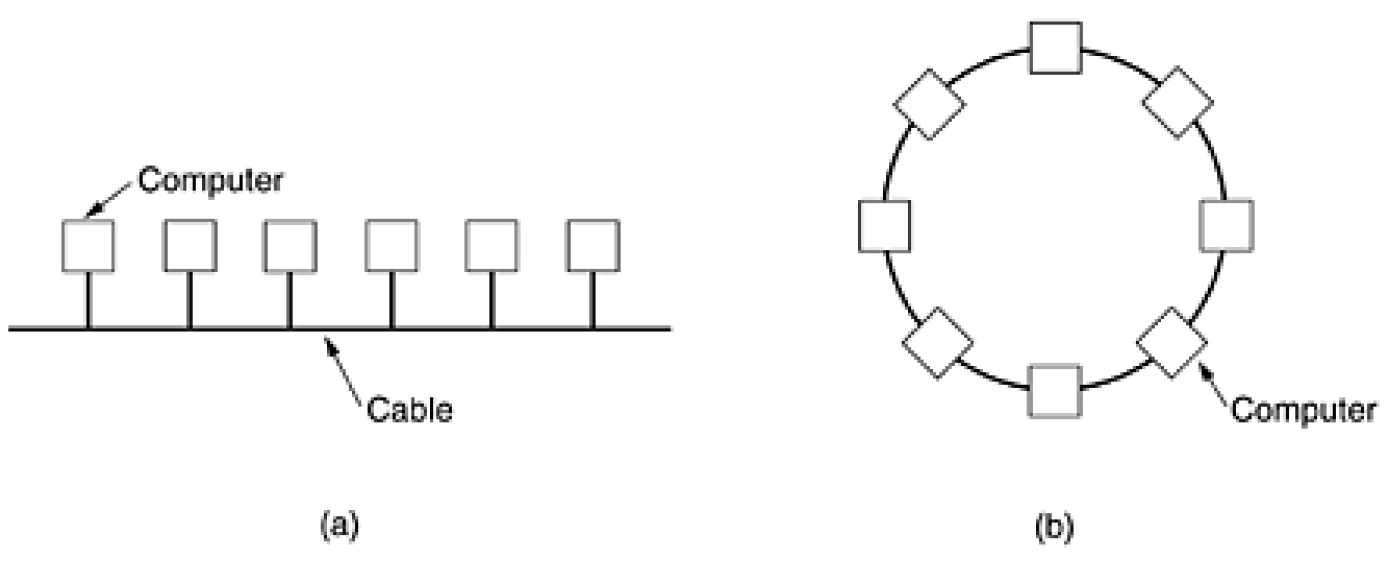
\includegraphics[width=1.0\textwidth]{chapters/ch-networks/figures/lan-networks-topologies}
  \caption{Two broadcast networks. (a) Bus. (b) Ring \cite{Tanembaum:2003cn}}
  \label{fig:lan-networks-topologies-fig}
\end{figure}

\section{Annotations}



\chapter{IEC 61850 Overview}

\section{Objects for distributed systems}

The effective distribution of Logical Nodes 
on diferents IEDs  
is a reality thanks to researches about 
the structure of distributed systems. More 
than 20 years ago emerged requirements 
for the object paradigm to suport the 
design and development of distributed systems.

Theses quotes were extracted from Jazayeri 
1988 research:

\emph{
``An object on one node can send a (multicast) message 
to several other objects \ldots''
} (MCAA) \todo{completar y ver si esta bien}

\emph{
`` \ldots The ability to group 
a set of objects and address them as one entity 
is important in many applications both from an 
efficiency point of view and from a program 
structuring point of view \ldots'' 
} (DO, DATA-SET, FCD, FCDA)\todo{completar y ver si esta bien}

\emph{
`` \ldots a final 
difference is that our objects are active and 
not reactive, in the sense that they can start 
up spontaneosly performing operations, not 
necessarily only in response to method invocations.
Such a facility is useful, for example, to allow objects 
to monitor the enviroment and change their behavior based 
on changes in the enviroment \ldots'' 
} (Some active objects 
are GOOSE, URCB and some passive object 
are \todo{completar y ver si esta bien})

\cite{Jazayeri:1988}.



\begin{figure}
  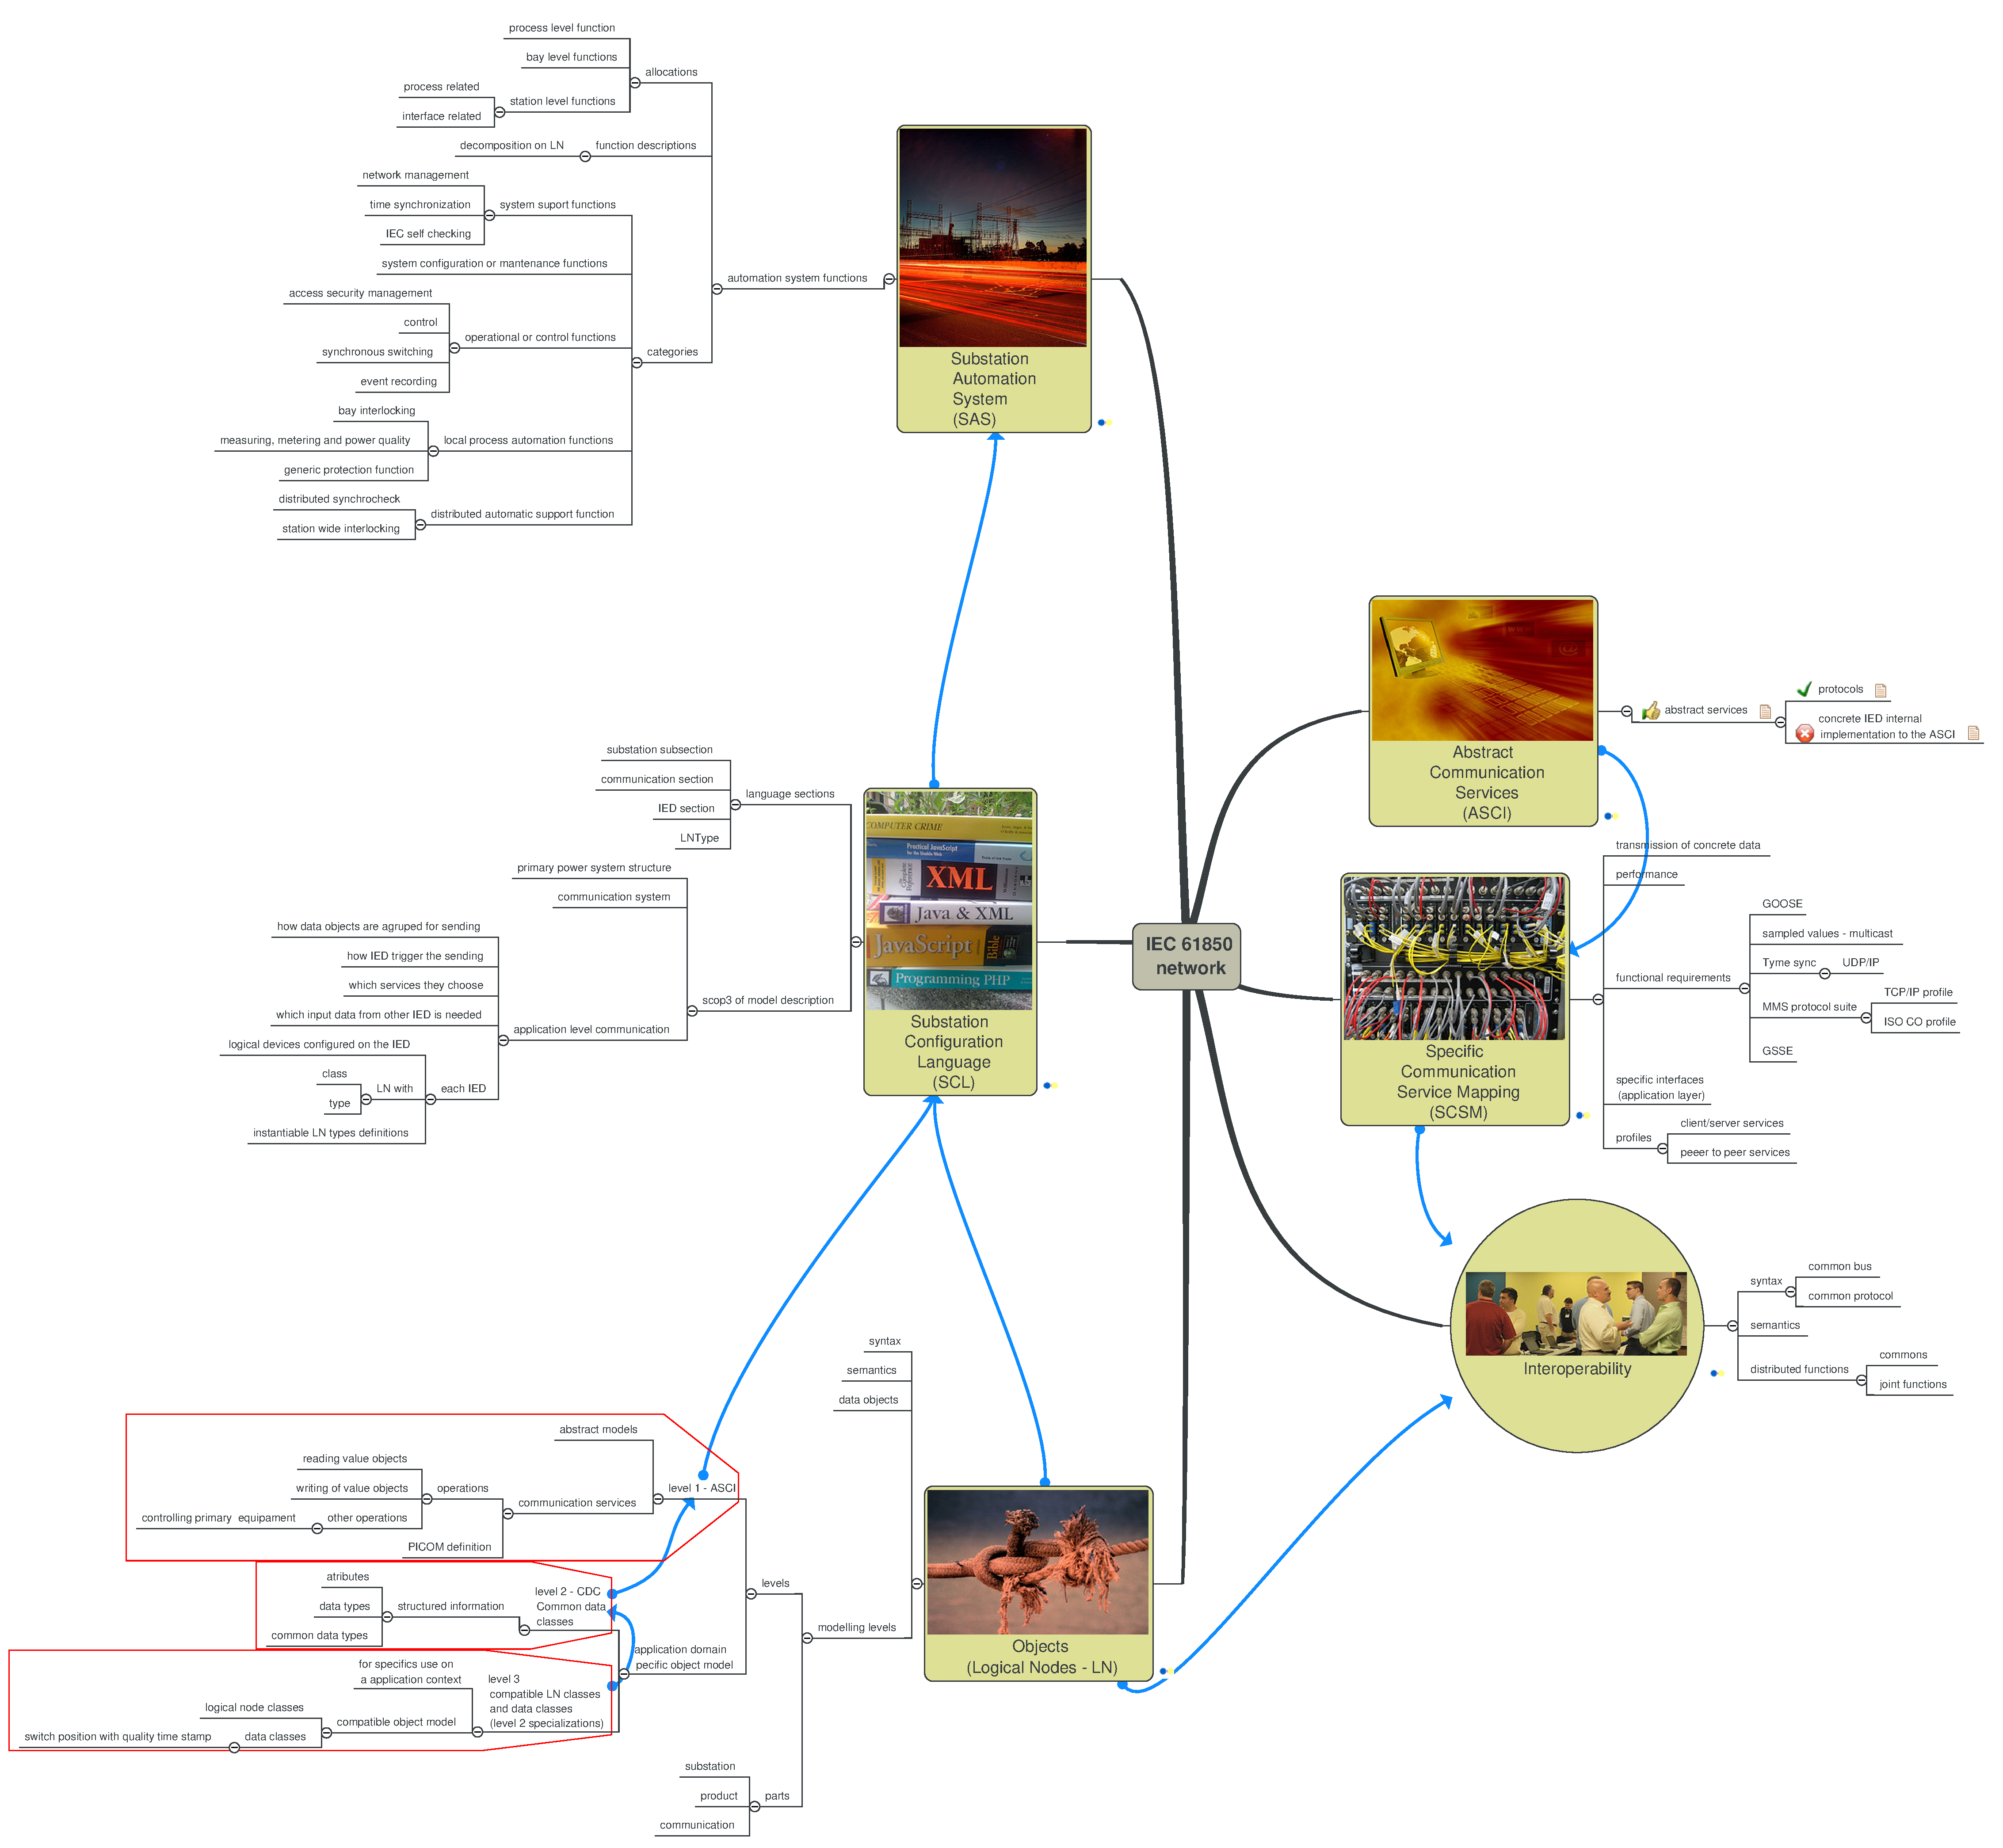
\includegraphics[width=1.0\textwidth]{appendices/IEC61850network}
  \caption{Borrador - Parte del esquema del futuro capitulo }
  \label{fig:lan-networks-topologies-fig1}
\end{figure}

\begin{landscape}
	\begin{figure}
	  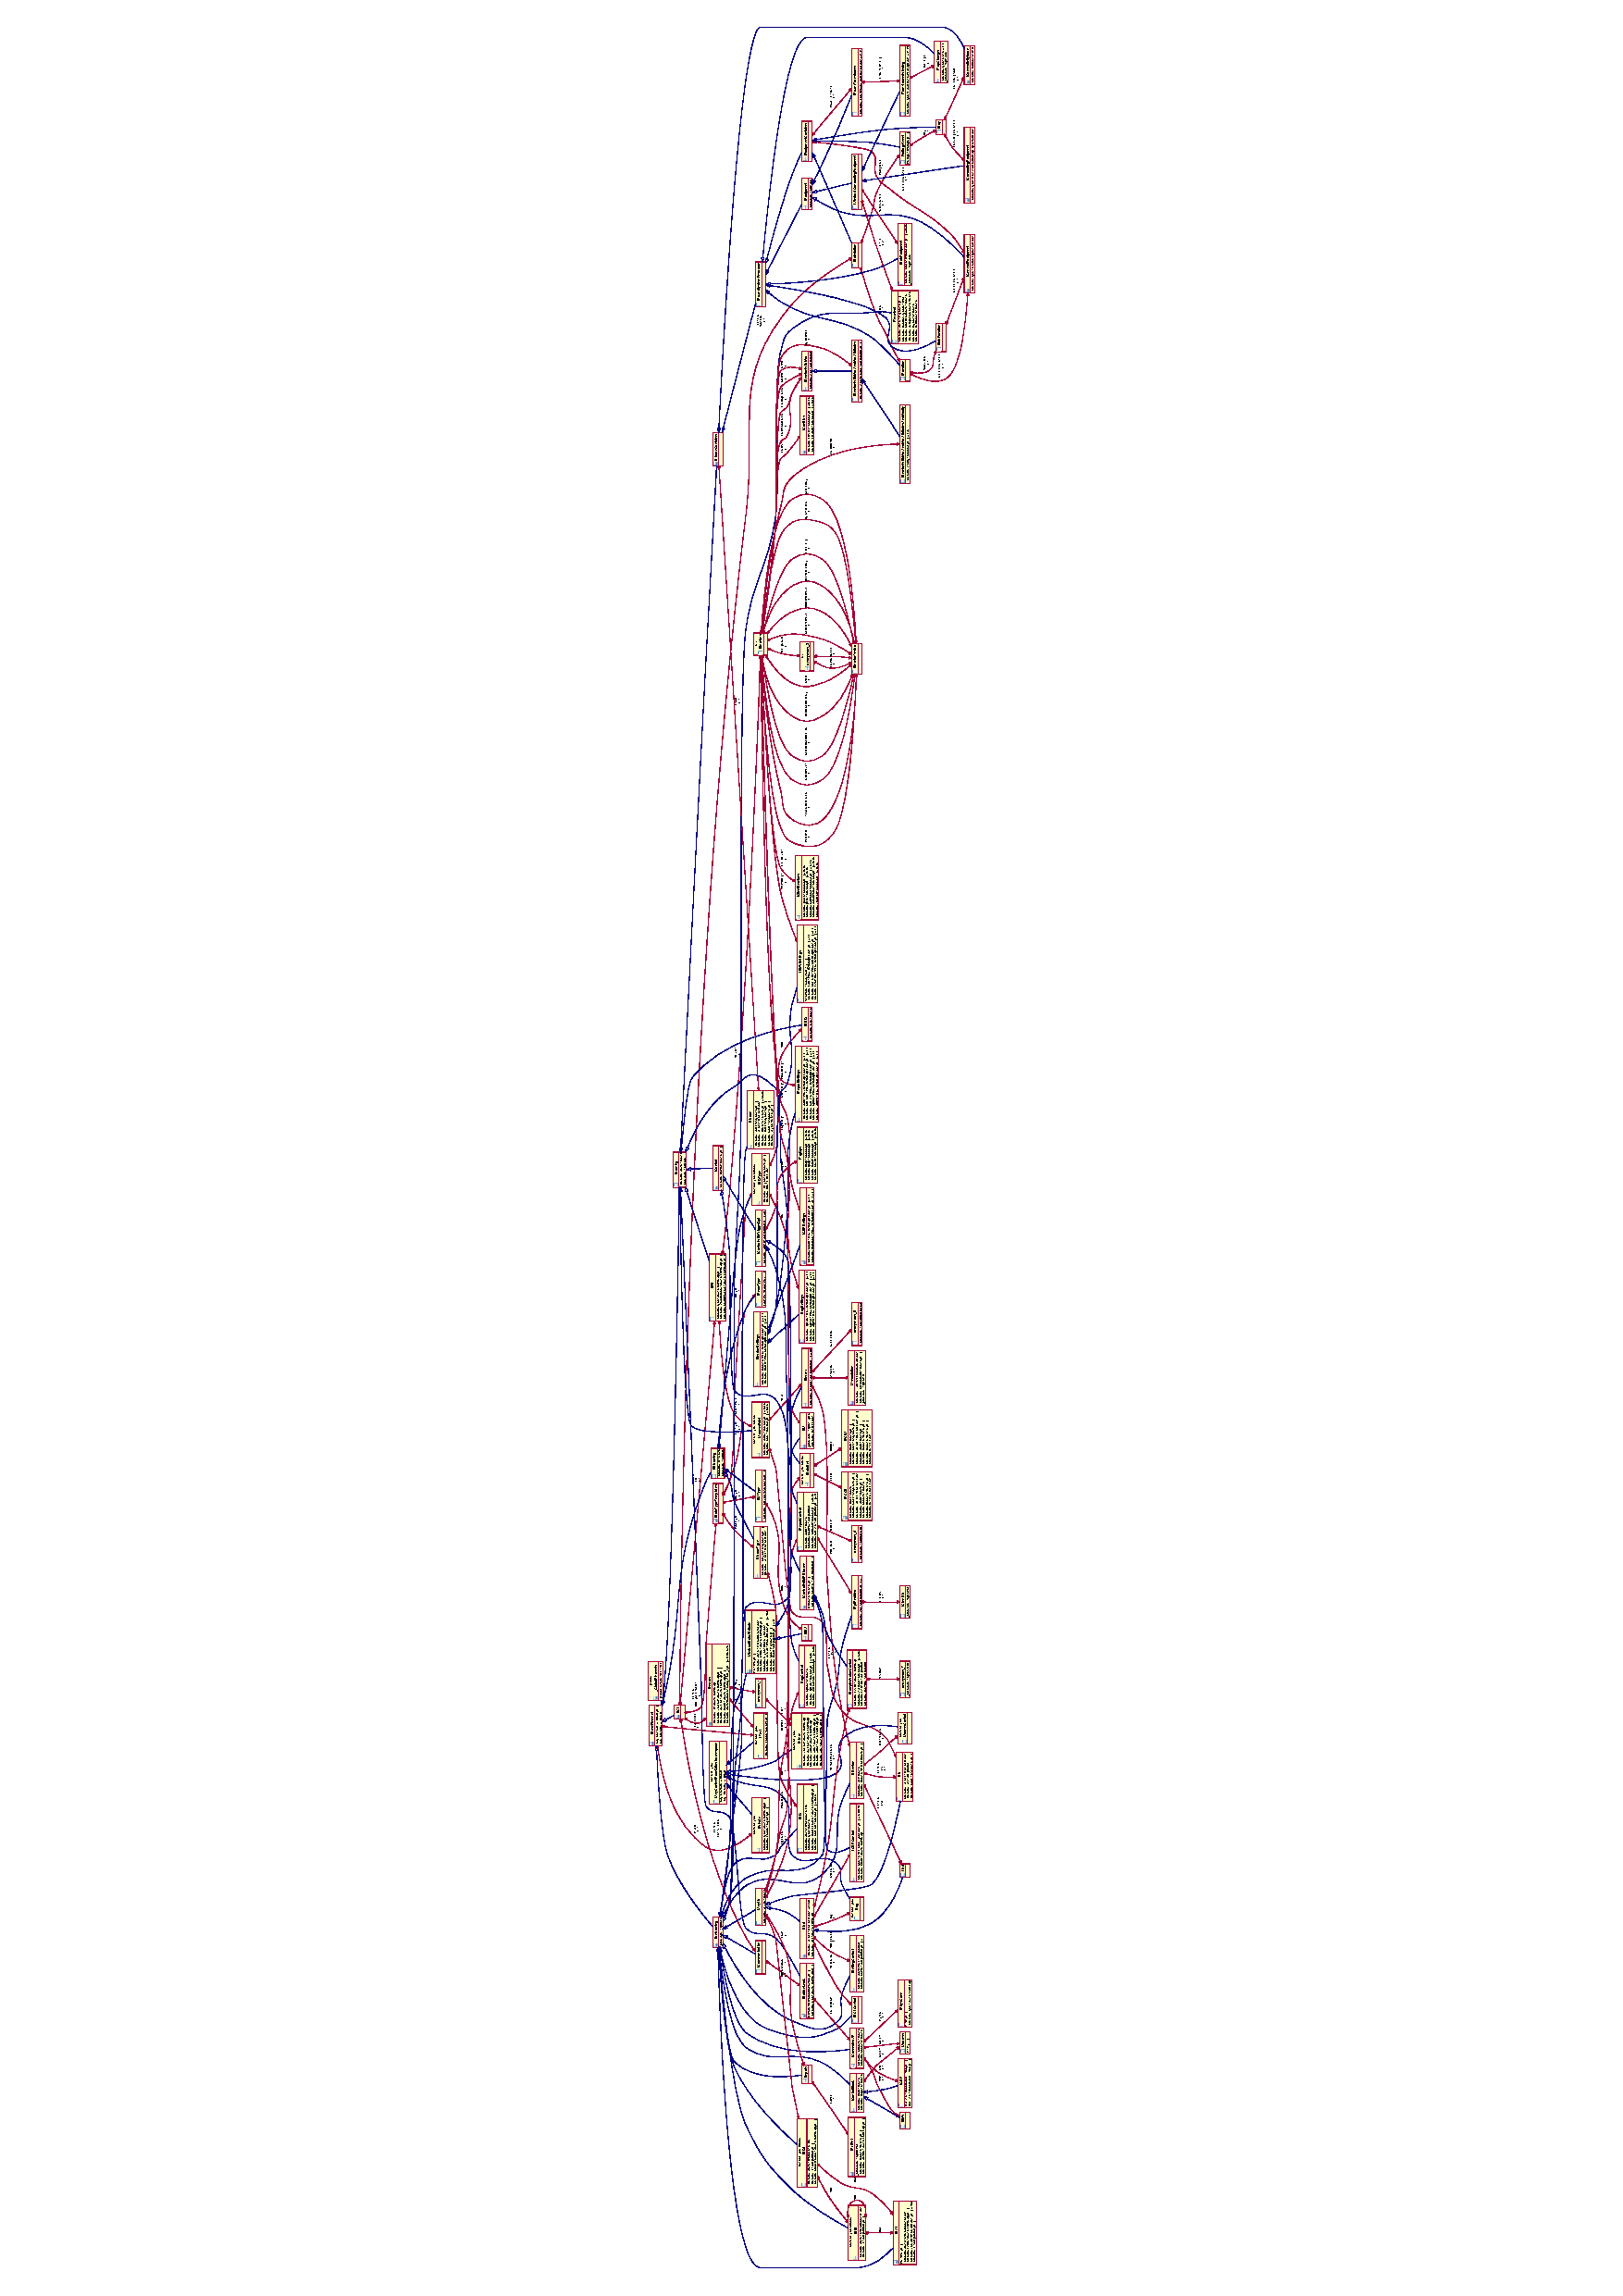
\includegraphics[angle=-90, width=1.0\linewidth]{appendices/JavaPrinting}
	  \caption{Borrador - Parte del esquema del futuro capitulo }
	  \label{fig:lan-networks-topologies-fig2}
	\end{figure}
\end{landscape}
 



\chapter{Substation Configuration Language}

\section{Introduction}

The \glspl{IED} in conformance with the 
IEC 61850 allow a communication related 
configuration with 
a standarized description language 
called \gls{SCL}, and they are specified 
in the part 6 of 
the IEC 61850 standard \cite{IEC61850-6:2004}.
The \gls{SCL} files, i.e., 
\gls{SCD}, \gls{ICD}, \gls{SSD} and \gls{CID} 
files describes an instance of the 
\gls{SCL} classes in a serialized form 
and standarized description of constraints and object structure. 
\todo[color=green!40]{61850, parte6, cl6.1, \textparagraph 3}

This chapter describes the model defined 
in the IEC 61850-6 \cite{IEC61850-6:2004}. This 
point of view will be useful for the 
nexts chapters where the Itaipu Hydro Power Plant 
functions will be modelled in conformance 
with this standard. 

All the classes described in this chapter are part 
of the IEC 61850-6 standard, and the SAS 
engineering are bounded to the right instantiation 
of the classes described here. A comprehensive explanation 
about \gls{O-O} systems (classes, instances and more) 
are provided in the chapter \ref{ch:ch-oop}.
In the standard, 
the classes mentioned above are represented 
by \gls{XSD} files,
and simplified \glspl{UML}. This chapter aims to 
provide a alternative approach for 
the understandability of the \gls{SCL} specification, 
%A good comprehension of the IEC 61850 Logical Nodes 
%and communication services models engineered 
%that result in a \gls{SCD} file 
\todo{aqui: revisar la gramatica}
describe the steps of the \gls{SCL} engineering 
and analyze a real case SCL by describing their 
more important parts, and providing the 
complete \gls{UML} class diagram of the IEC 61850-6.




\section{SCL engineering parts} \label{sec:SCL-engineering-parts}

The SCL description capability are 
an important \gls{SAS} engineering part, and may
start either with the SAS functional specification, 
\gls{IED} capability description or with the 
\gls{SAS} description. Theses steps 
are explained 
in the following subsections: 

\subsection{SAS functional specification}
The functional specification input to \gls{SAS} engineering 
consist in the system specification in terms of 
single line diagram, allocation of the \glspl{LN} 
and equipmets of the single line.

\subsection{IED capability description}
Another right name for this step is IED pre-engineering. 
In this step are described the IED capabilityes, for 
example, a IED with the double busbar line feeder function.

\subsection{SAS description}
This is part of the \gls{SAS} engineering, where the 
complete process configuration takes place: All IED 
are bounded to individual process functions and primary 
equipments, enhanced by access point connections and 
the access path in subnetworks for the clients.

A complete \gls{SAS} description provides 
all predefined associations and client-server connections 
(the \gls{IED} cannot built it automatically).

\todo[inline]{ver como puedo ir concatenando las ideas, hasta
desenvocar en este diagrama de secuencia}
A more detailed description are provided by this UML secuence diagram.

\begin{figure}
  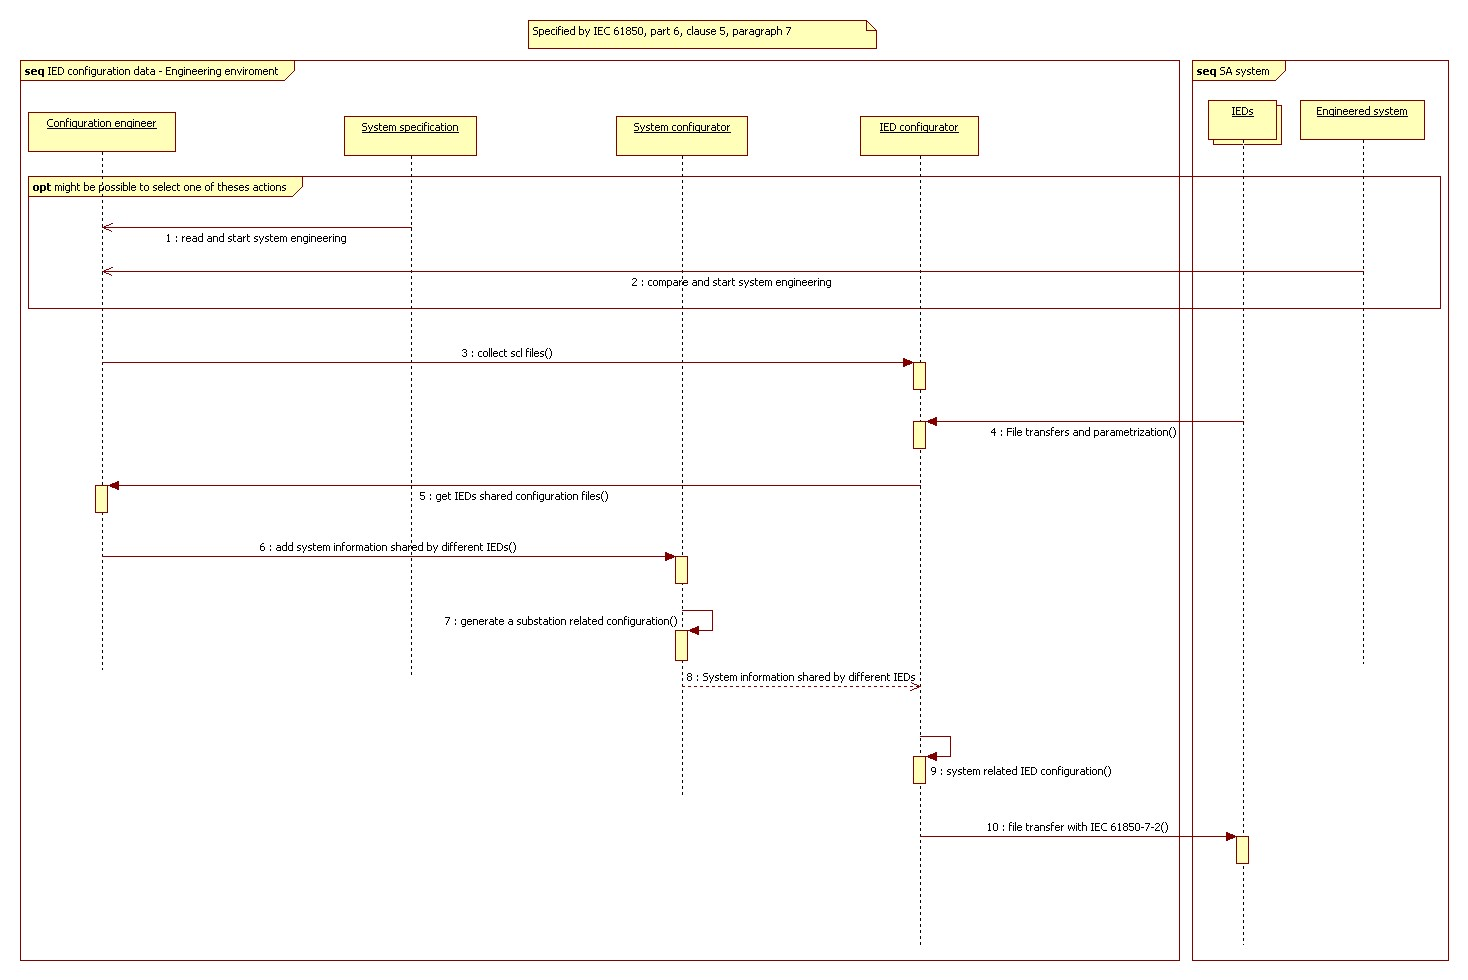
\includegraphics[width=1.0\textwidth]{chapters/ch-scl/figures/SCL-development-process}
  \caption{SCL engineering process}
  \label{fig:SCL-development-process}
\end{figure}


\section{Tools}

According to the functionality, the tools for 
SCL engineering steps 
mentioned in section \ref{sec:SCL-engineering-parts} are
classified in the IEC 61850-6 \cite{IEC61850-6:2004} as
follows:

\subsection{IED configurator tool}
Support SCL importing and exporting generating IED specific 
configuration files and providing IED specific settings.

\subsection{System configurator tool}
\label{sec:ch-scl--System-configurator-tool}
The system configuration tool in conformance
with the IEC 61850-6 \cite{IEC61850-6:2004} can import 
configuration files from several \glspl{IED}, 
export configuration files and generate 
substation related configuration files.

The are tools used for the engineering steps 
mentioned in section  
and they are 


\section{SCL conformace}
%\section{SCL conformace in the IEC 61850 context}

The SCL files shall be validate with the 
\glspl{XSD} defined by the 
IEC 61850-6 \cite{IEC61850-6:2004} , and 
the IEDs shall handle theses SCL files 
in conformance with the specification.
The responsibilities listed below are 
defined by \cite[clause 5]{IEC61850-6:2004}. %paragraph 7

	\subsection{The IED responsability for SCL handling}
	\begin{itemize}
		\item 	The IED shall describe their capabilities by providing 
	 			the SCL file or it shall provide a external tool which 
	 			can generate the SCL file from the IED. 
	 	\item	The IED shall contain a alternative to setup the 
	 			communication: 
	 			
	 			\begin{itemize} 
                   \item Can use a system SCL file or 
                   \item can be accompained by a external 
                   		 tool which can import 
	 					 a two-party tool generated SCL file to the IED.
	 			\todo[inline]{al decir two party me 
	 			refiero a heramientas
	 			 de otras empresas, no se si se dice two-party 
	 			 o third-party.}
	 			 \end{itemize}
    \end{itemize}
 	 

\section{SCL object model}
\label{sec:ch-scl--SCL-object-model}
As explained in the section \ref{sec:ch-scl--SCL-definition}, 
the SCL describes the SAS by modelling objects.
The standard IEC 61850-6 \cite{IEC61850-6:2004} object model 
structure and constraints are described in terms of the 
\gls{XSD}.

The \gls{XSD} of the \gls{SCL} are structured as depicted 
in the figure \href{fig:pdf-SCL-uml-deept2}. 

\begin{center}
	\begin{figure}
	  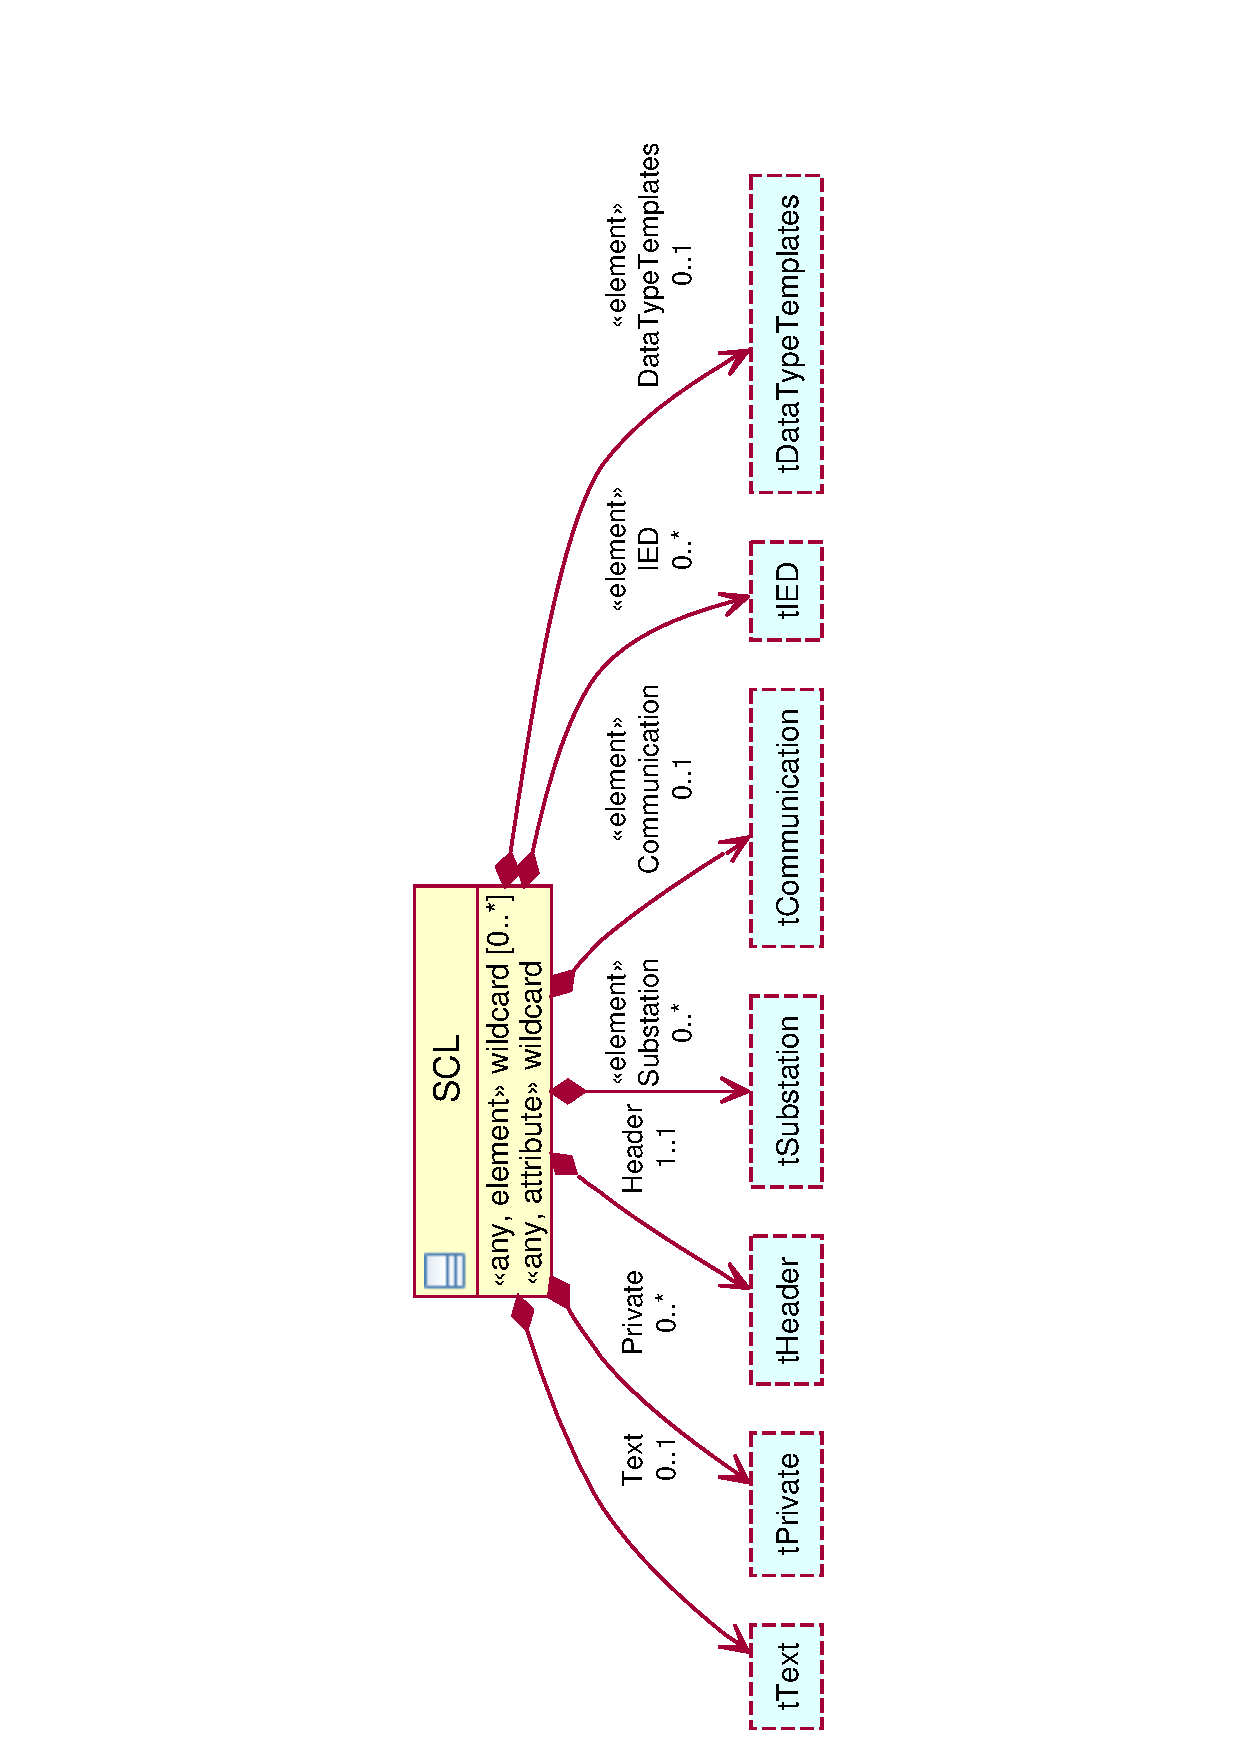
\includegraphics[
						angle=-90,	  
	  					width=1.0\textwidth 
	  				   ]{chapters/ch-scl/figures/SCL-uml-Deept2}
	  \caption{SCL object model}  
	  \label{fig:pdf-SCL-uml-deept2}
	\end{figure}
\end{center}
 
%\begin{landscape}
%\end{landscape}


Basically, it is composed by: 
\todo[color=green!40]{61850, parte6, cl6.1, \textparagraph 5}



\begin{itemize}
  \item The substation model: the object model of the primary power structure
  		(a instance of tSubstation) with their designations structured according to 
  		IEC 61346-1 \cite{IEC61346-1:1996}. 
  \item The communication model: the object model of the IED 
  		communication system configuration, 
  		i.e.,
  		the the networks, subnetworks, ports informations
  		\todo[color=green!40]{61850, parte6, cl6.1, \textparagraph 5},
  		the communication connection relations of IEDs to 
  		subnetworks, the routing for another subnetworks informations, 
  		and clocks configuration information and locations for 
  		time synchronisation (the gateways are not considered here, 
  		a gateway has to be modelled as another IED)
  		\todo[color=green!40]{61850, parte6, cl6.1, \textparagraph 8}.
  \item The product model: Contains the IEDs objects and their 
  		logical node implementations. 
  \todo[inline]{averiguar la funcion del DataTypeTemplates para agregar aca
  si corresponde}
\end{itemize}

All the structures are derived from differents 
parts depicted in the figure \ref{fig:pdf-SCL-uml-deept2}. 
In this figure, each class represent the top level 
of their structure, e.g., the substation class 
mentioned here has voltage levels, 
connectivity nodes and tranformers.   
Theses classes are completely decoupled 
(the most notable decoupling are the diferentiation of  
Logical node classes on the 
IED -t\gls{LN}- and Substation -t\gls{LNode}- structure), 
allowing the separation of the \gls{SCL} development 
by the differents engineering process 
described in the section \ref{sec:SCL-engineering-parts}.


The \gls{SCL} relationship are based in a 
ring \gls{O-O} architecture between Substation,
IED, Header, Communication, and DataTypeTemplate classes,
and it are based in a hierarchical structure under each of the 
mentioned classes.



\subsection{SCL modelling steps}
\todo[inline]{esta seccion la dejo pendiente,
debo escribirlo con detenimiento para 
que queden en concordancia la 
figura \ref{fig:pdf-SCL-uml-deept2} 
y lo que tengo escrito en esta seccion}

The figure \ref{fig:SCL-development-process} 
show the detailed SAS engineering 
process depicted with 
the autor interpretation of the step 
mentioned in the standard by 
using an \gls{UML} secuence diagram.

The more usual approach for the \gls{SAS} description 
with \gls{SCL} begin with the 
single line drawing process where the 
substation topology are defined using a 
system configurator tool. The system configurator tool, 
described in the section \ref{sec:ch-scl--System-configurator-tool}, 
creates the \gls{SSD} file containing the \glspl{LNode}
and their allocation in the substation. 
The class diagram provided by the author 	 
are based on the \gls{SCL} 
\gls{XSD}['s] of the substation. (figures  
\ref{fig:pdf-SCL-uml-substation-Deept2} and 
\ref{fig:pdf-SCL-uml-substation-Deept2-inherited}).

The \glspl{LNode} objects SCL models 
(from the substation section) is used to map 
the \gls{IED} object model references  
(figure \ref{}
\todo{apuntar a label{fig:pdf-SCL-uml-IED-Deept2}}) 
that describes 
the \gls{IED} objects are used to mapping 
\todo{terminar bien este parrafo\ldots}


\todo[inline]{a este le falta
expandir la clase correspondiente hasta que muestre el transformador }
\begin{figure}
  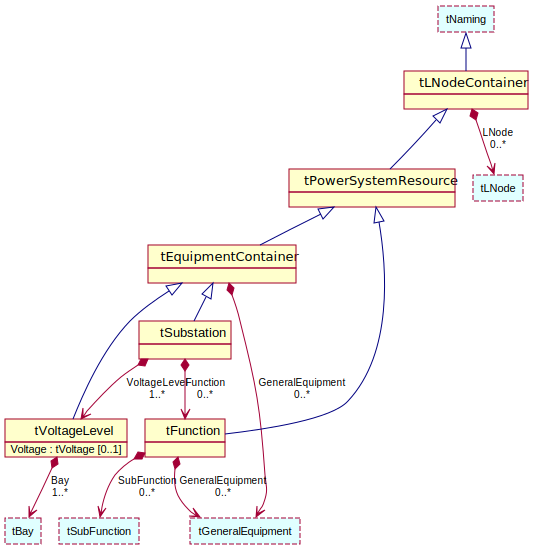
\includegraphics[width=1.0\linewidth]{chapters/ch-scl/figures/SCL-uml-substation-Deept2}
  \caption{SCL Substation class diagram with heritance 
  details} 
  \label{fig:pdf-SCL-uml-substation-Deept2}
\end{figure}


\todo[inline]{a este le valta
  expandir la clase correspondiente hasta que muestre el transformador }
\begin{figure}
  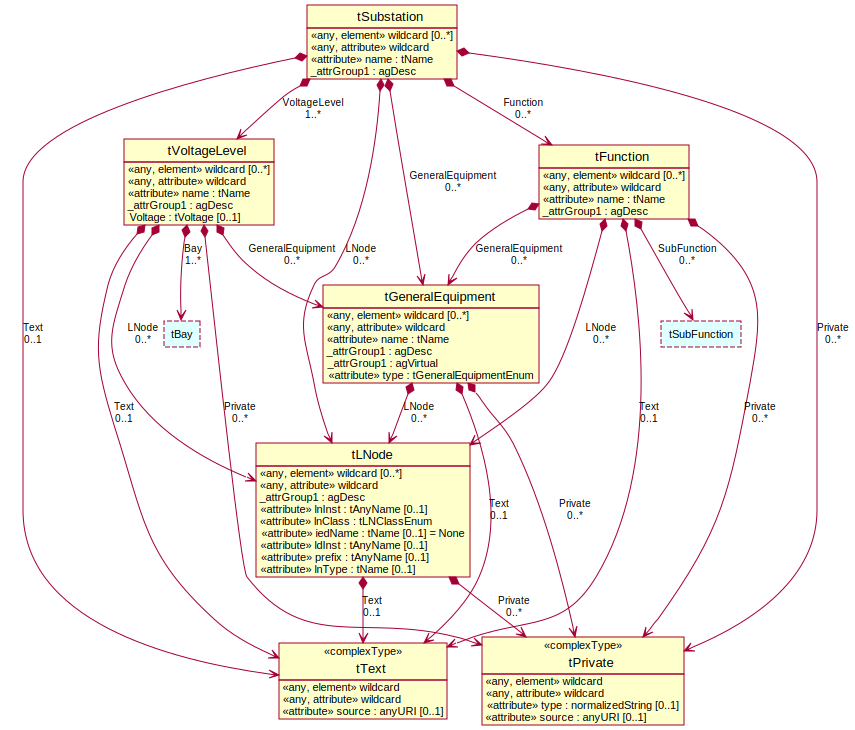
\includegraphics[width=1.0\linewidth]{chapters/ch-scl/figures/SCL-uml-substation-Deept2-inherited}
  \caption{SCL Substation class diagram inherited  }
  \label{fig:pdf-SCL-uml-substation-Deept2-inherited}
\end{figure}


\begin{figure}
  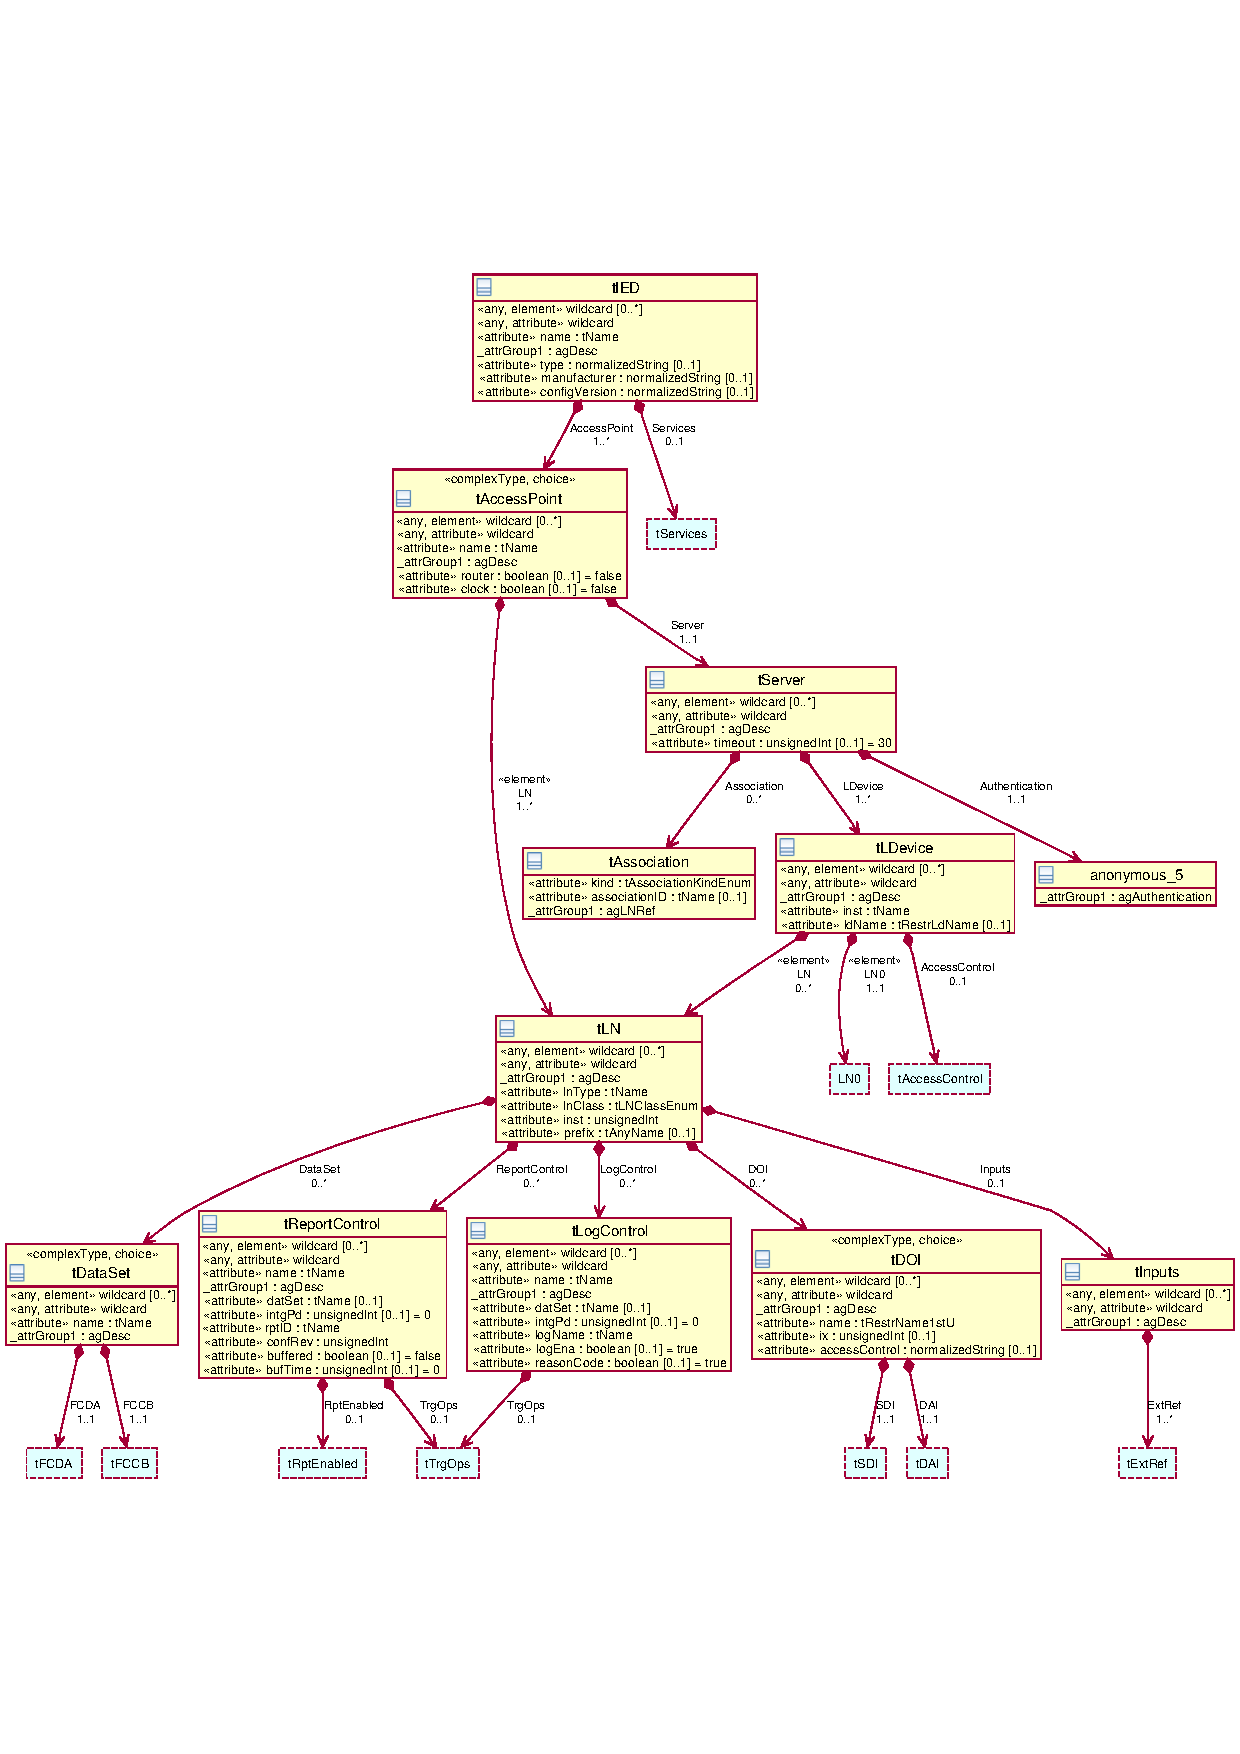
\includegraphics[width=1.0\linewidth]{chapters/ch-scl/figures/SCL-uml-IED-Deept2-inherited}
  \caption{SCL Substation class diagram inherited  }
  \label{fig:pdf-SCL-uml-IED-Deept2-inherited}
\end{figure}

%\begin{figure}
% 
%  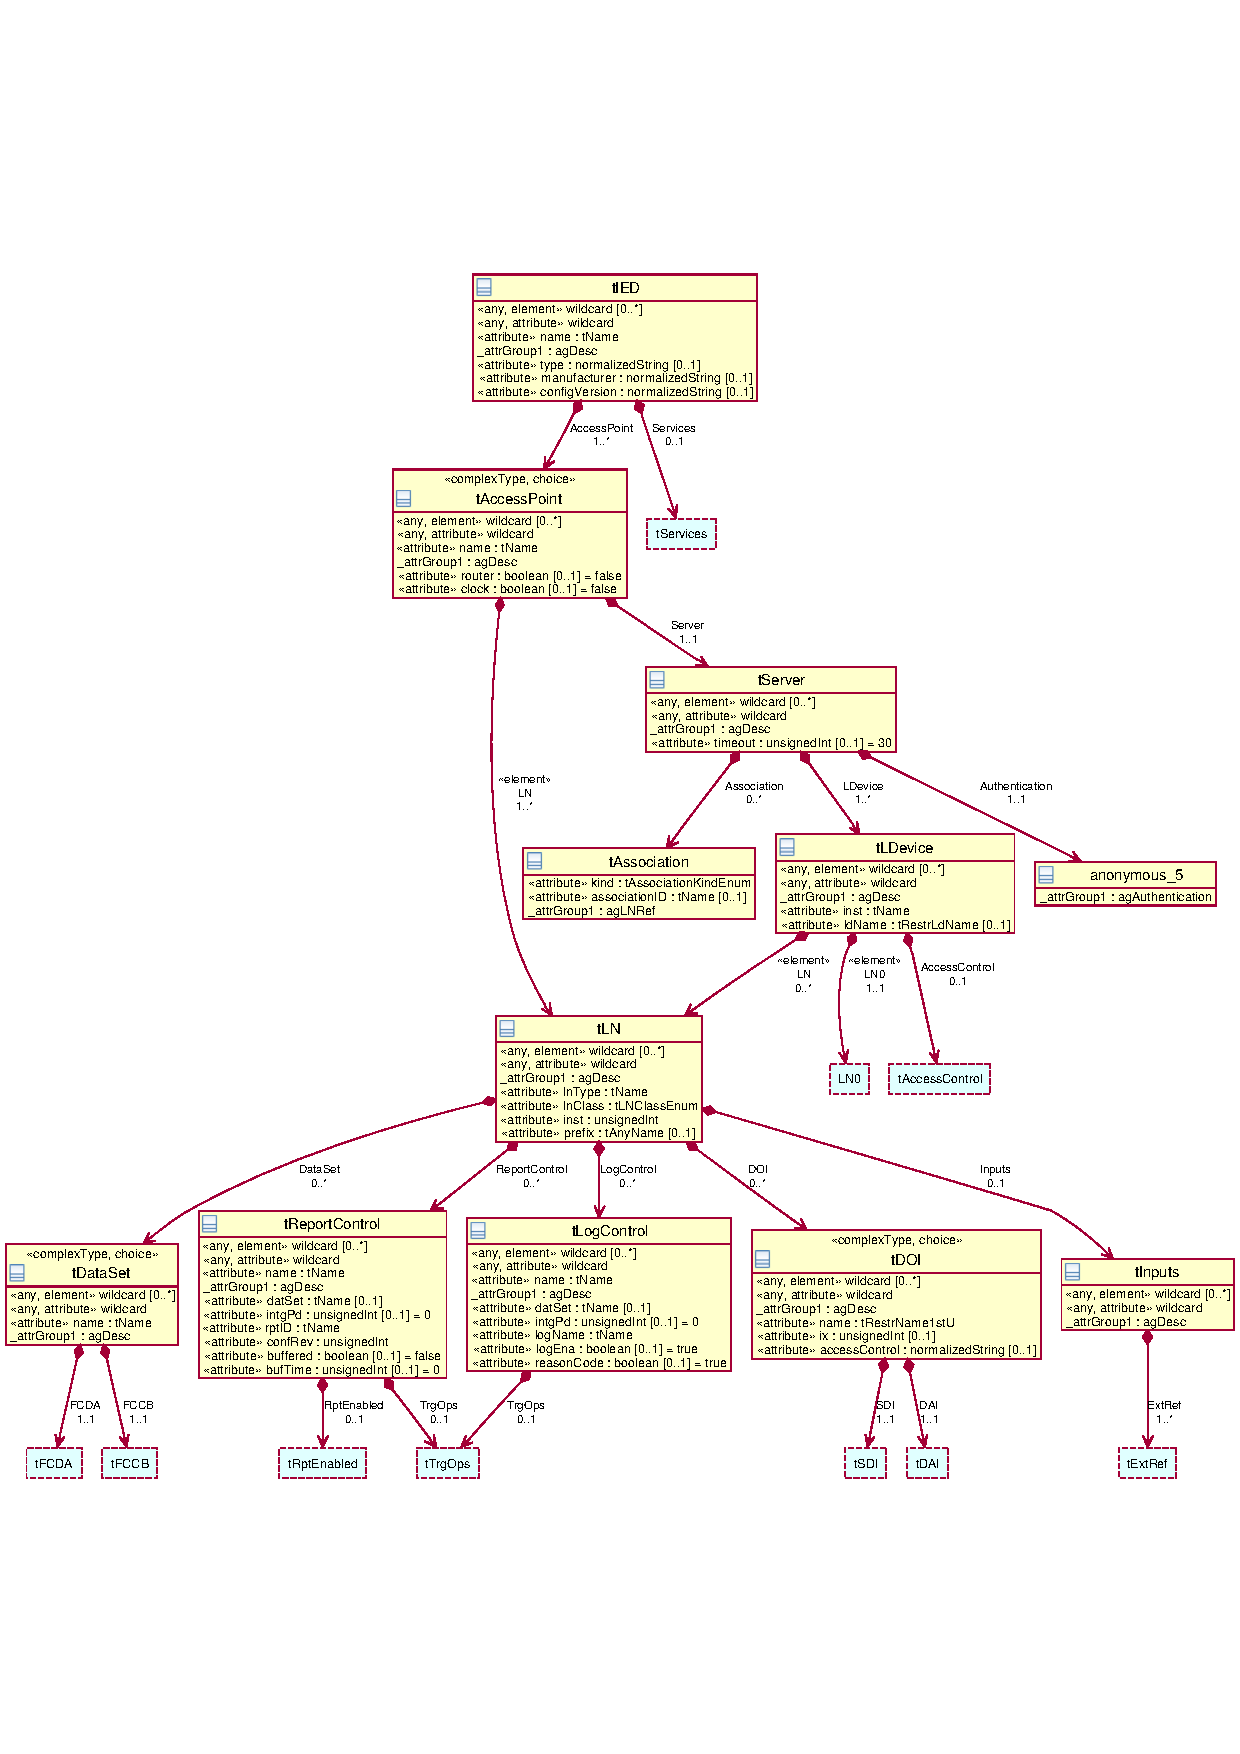
\includegraphics[width=1.0\linewidth]{chapters/ch-scl/figures/SCL-uml-IED-Deept2-inherited}
%  \caption{SCL Substation class diagram inherited  }
%  \label{fig:pdf-SCL-uml-IED-Deept2}
%\end{figure}
\missingfigure[color=green!40]{aqui falta el uml del IED con detalles de
herencia}



\todo[inline]{debo agregar aca la explicacion de los demas modelos
descriptos mediance los XSDs, pues esos tres 
items que menciona la norma son solo los mas
importantes, pero no da para entender y saber leer 
los archivos scl sabiendo solo eso. Los tres items mencionados arriba
son solo la base. Falta principalmente el DATypeTemplate
que corresponden a los objetos a serializar correspondientes 
a las instancias de las clases de la parte 7-x}



\begin{landscape}
	\begin{figure}
	  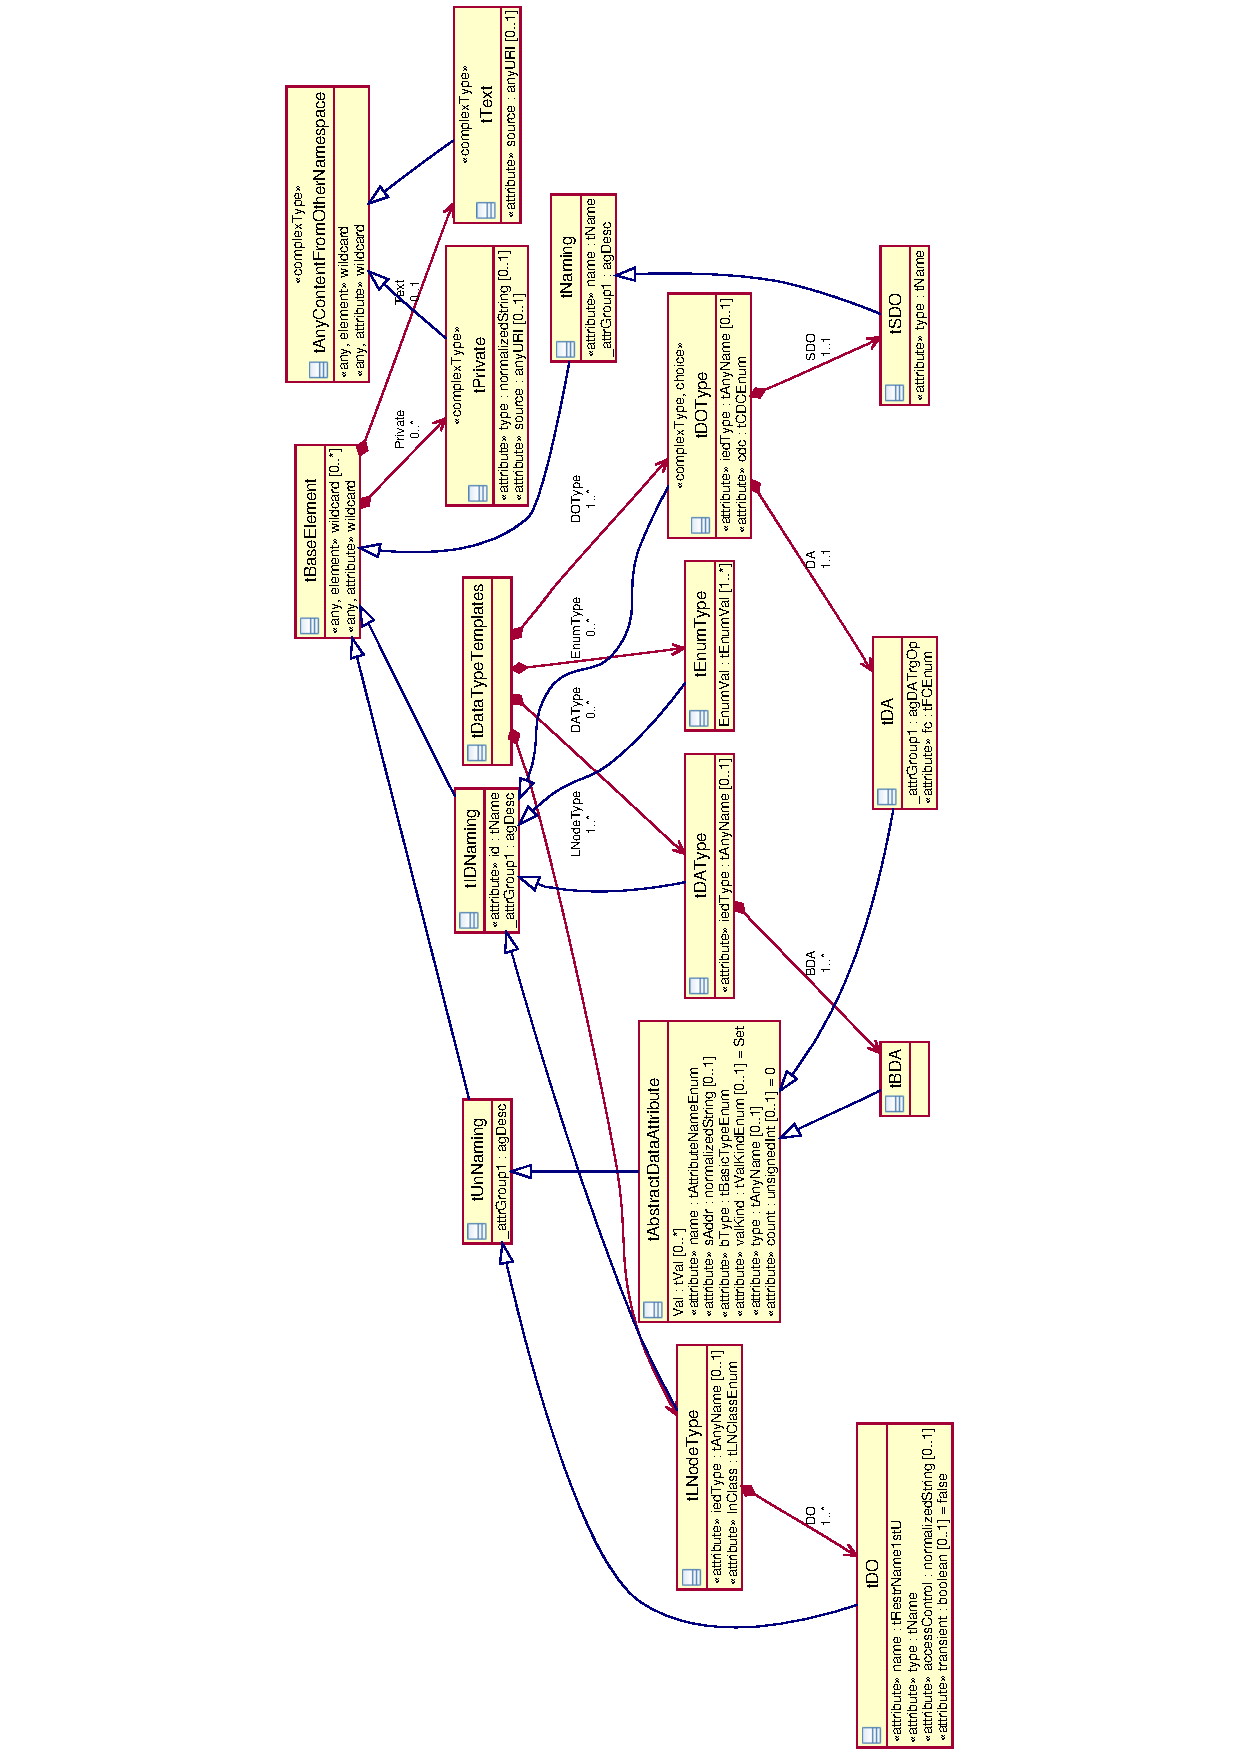
\includegraphics[angle=-90, width=1.0\linewidth]{chapters/ch-scl/figures/SCL-uml-DATypeTemplate-Deept2}
	  \caption{DAType class diagram template with heritance details}  
	  \label{fig:pdf-SCL-uml-DATypeTemplate-Deept2}
	\end{figure}
\end{landscape}

\begin{landscape}
	\begin{figure}
	  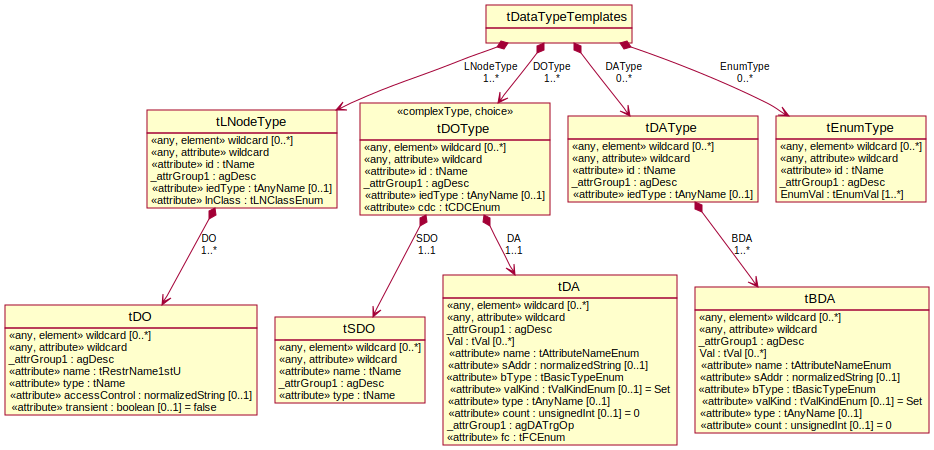
\includegraphics[angle=-90, width=1.0\linewidth]{chapters/ch-scl/figures/SCL-uml-DATypeTemplate-Deept2-inherited}
	  \caption{DAType class diagram template inherited}  
	  \label{fig:pdf-SCL-uml-DATypeTemplate-Deept2-inherited}
	\end{figure}
\end{landscape}

\begin{landscape}
	\begin{figure}
	  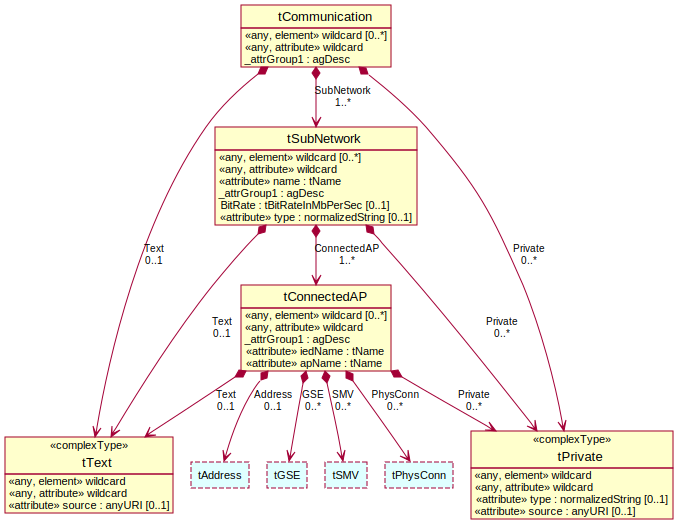
\includegraphics[angle=-90, width=1.0\linewidth]{chapters/ch-scl/figures/SCL-uml-communication-Deept3}
	  \caption{SCL Communication class diagram}  
	  \label{fig:pdf-SCL-uml-communication-Deept3}
	\end{figure}
\end{landscape}


The UML of the 
figure \ref{fig:SCL-uml-Resumen} 
is a resume of
the SCL model, where is evident the 
key importance of the Logical Node for  
the information topology description (see 
the composition of the Substation 
class). The Logical Node is  
the transition object to 
connect the diferent structures of the SAS 
\todo[color=green!40]{61850, parte6, cl6.1, \textparagraph 9} 
that are defined by IEC 61341-1 \cite{IEC61346-1:1996}.


\begin{landscape}

\begin{figure}
  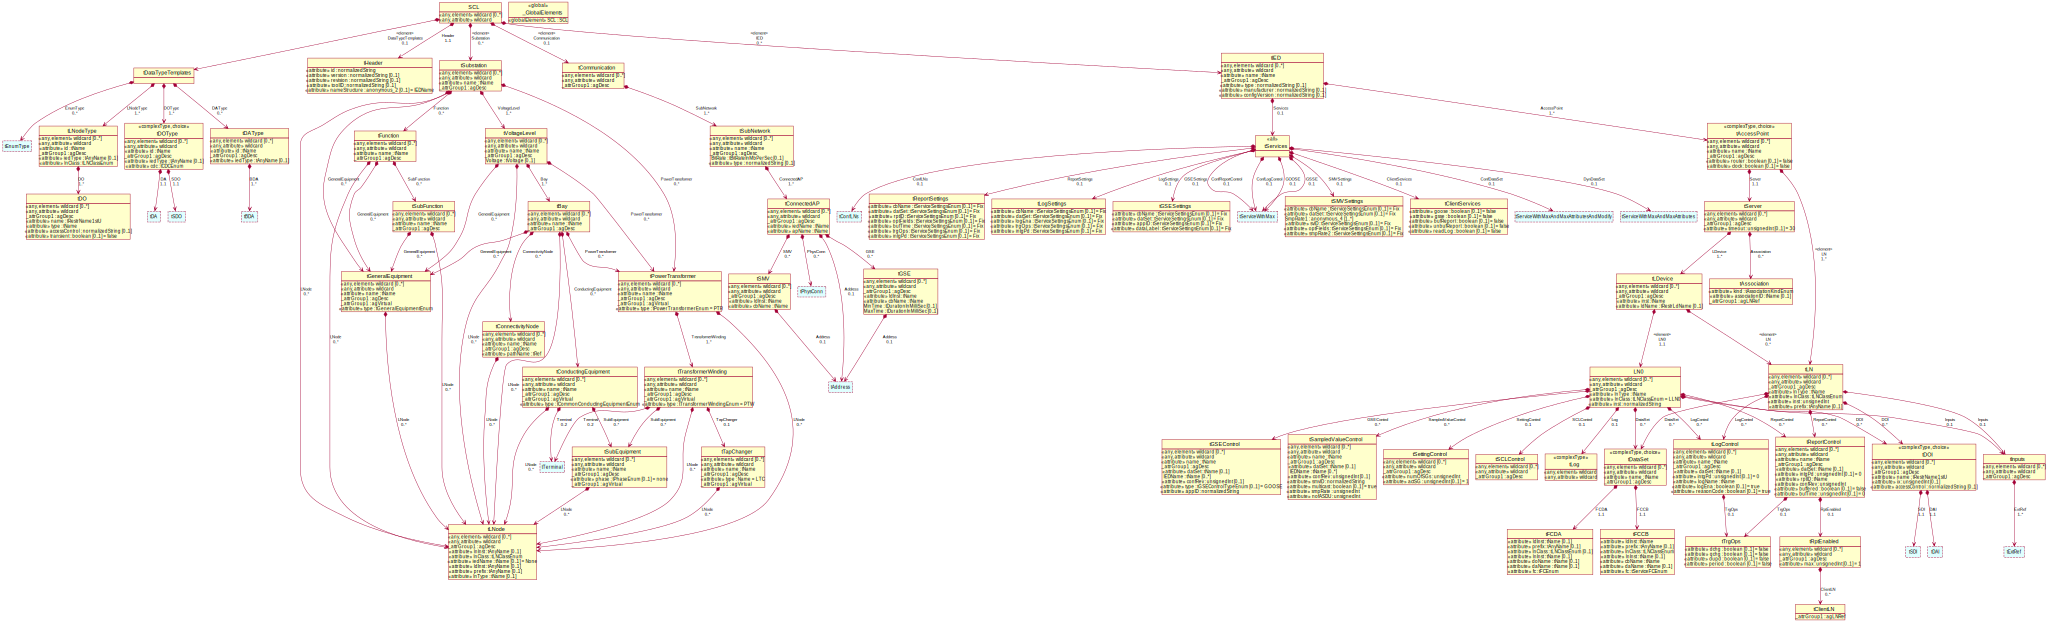
\includegraphics[angle=-90,
  width=1.0\linewidth]{chapters/ch-scl/figures/SCL-uml-Resumen-inherited}
  \caption{Resume of SCL shema represented by a UML class diagram}
  \label{fig:SCL-uml-Resumen}
\end{figure}
\end{landscape}

\section{SCL sections}

\begin{itemize}
  \item The SSD contains a header and a substation sections.
  \item The ICD contains a header, IED, and optionally a Substation template
  		sections.
  \item The SCD contains a header, substation, communication, multiple IEDs and 
  		multiple Data Type Templates.
  \item The CID contains a header, IEDs and their values, one instance 
  		of communication, and optionally a substation section. 
\end{itemize}

 


\appendix
\chapter{Tables}

\begin{table}
\caption{Armadillos}
\label{arm:table}
\begin{center}
\begin{tabular}{||l|l||}\hline
Armadillos & are \\\hline
our	   & friends \\\hline
\end{tabular}
\end{center}
\end{table}

\clearpage
\newpage

\chapter{Figures}

\vspace*{-3in}

\begin{figure}
\vspace{2.4in}
\caption{Armadillo slaying lawyer.}
\label{arm:fig1}
\end{figure}
\clearpage
\newpage

\begin{figure}
\vspace{2.4in}
\caption{Armadillo eradicating national debt.}
\label{arm:fig2}
\end{figure}
\clearpage
\newpage

\begin{singlespace}



%esta es la bibliografia standard de la IEEE
\bibliographystyle{IEEEtran}
\bibliography{IEEEabrv,bibliography/myIEEEbibliography}
%\bibliographystyle{plain}
%\bibliography{bibliography/myIEEEbibliography}

%\bibliography{main}
%\bibliographystyle{plain}
\end{singlespace}
\end{document}

